% %
% LAYOUT_E.TEX - Short description of REFMAN.CLS
%                                       99-03-20
%
%  Updated for REFMAN.CLS (LaTeX2e)
%
\documentclass[8pt]{refart}
\usepackage{makeidx}
\usepackage{ifthen}
\usepackage{amsmath}
\usepackage{amsfonts}
\usepackage{amssymb}
\usepackage[langlinenos]{minted}
\usemintedstyle{manni}
\usepackage{url}
\usepackage[backend=bibtex,style=numeric]{biblatex}
\addbibresource{bib.bib}  
\usepackage{mhchem}
\usepackage{hyperref}
\hypersetup{
    colorlinks=true,
    linkcolor=blue,
    filecolor=yellow,      
    urlcolor=magenta,
}
\usepackage{listings}
\usepackage{xparse}
\usepackage{amsfonts}
\usepackage{enumitem}
\usepackage{bbm}
\usepackage{amssymb}
%\usepackage{parskip}
\NewDocumentEnvironment{code}{ O{1} o o m }
{
  \VerbatimEnvironment
  \begin{listing}[H]
  \IfNoValueTF{#2} {} {\caption{#2}}
  \IfNoValueTF{#3} {} {\label{#3}}
  \begin{minted}[
  frame=single,
  firstnumber=#1,
  framesep=2mm,
  baselinestretch=1.2,
  fontsize=\footnotesize,
  linenos,
  breaklines]{#4}
}
{
  \end{minted}
  \end{listing}
  \vspace*{-2\baselineskip}
}
\NewDocumentEnvironment{codenolinenums}{ O{1} o o m }
{
  \VerbatimEnvironment
  \begin{listing}[H]
  \IfNoValueOrEmptyTF{#2} {} {\caption{#2}}
  \IfNoValueOrEmptyTF{#3} {} {\label{#3}}
  \begin{minted}[
  frame=single,
  firstnumber=#1,
  framesep=2mm,
  baselinestretch=1.2,
  fontsize=\footnotesize,
  breaklines]{#4}
}
{
  \end{minted}
  \end{listing}
  \vspace*{-2\baselineskip}
}
% code example
% \begin{code}[10][Python example][python_example]{python}
% from etraj import Matrix
% for i in range(10):
%     x = 5
%     for j in range(x):
%         print(i,j)
% \end{code}

\usepackage{makecell}
\newcommand\gobbleone[1]{}
\newcommand*{\seeonly}[2]{\ (\emph{\seename} #1)}
\newcommand*{\also}[2]{(\emph{\alsoname} #1)}
\newcommand{\Also}[2]{\emph{See also} #1}
\usepackage{fancyhdr}
\usepackage{graphicx}
\usepackage[graphicx]{realboxes}
%\usepackage{geometry}
\pagestyle{fancy}
\fancyhf{}
\let\Sectionmark\sectionmark
\def\sectionmark#1{\def\Sectionname{#1}\Sectionmark{#1}}
\let\Subsectionmark\subsectionmark
\def\subsectionmark#1{\def\Subsectionname{#1}\Subsectionmark{#1}}
\let\Subsubsectionmark\subsubsectionmark
\def\subsubsectionmark#1{\def\Subsubsectionname{#1}\Subsubsectionmark{#1}}
%\fancyhead[LE,RO]{\rightmark}
\fancyhead[RE, LO]{Guides and Tutorials: Neutron Calibration}
\fancyfoot[CE, CO]{\thesubsection.\ \Subsectionname}
\fancyfoot[LE, RO]{\thepage}
\renewcommand{\headrulewidth}{2pt}
\renewcommand{\footrulewidth}{1pt}
\usepackage{lscape}

\urlstyle{same}


\def\bs{\char'134 } 
\newcommand{\ie}{i.\,e.,}
\newcommand{\eg}{e.\,g..}
\DeclareRobustCommand\cs[1]{\texttt{\char`\\#1}}

\title{Neutron Calibration on DUNE}
\author{Nicholas Carrara$^1$\thanks{ncarrara.physics@gmail.com}, Yashwanth Bezawada$^1$\thanks{ysbezawada@ucdavis.edu}, Junying Huang$^1$\thanks{jyghuang@ucdavis.edu}\\Jingbo Wang$^2$\thanks{jingbo.wang@sdsmt.edu}, Walker Johnson$^2$\thanks{walker.johnson@mines.sdsmt.edu}\\
Robert Svoboda$^1$\thanks{rsvoboda@ucdavis.edu}, Michael Mulhearn$^1$\thanks{mjmulhearn@ucdavis.edu}\\
${}^1$University of California at Davis, Physics Department, Davis, CA 95616\\
${}^2$South Dakota School of Mines \& Technology, Physics Department, Rapid City, SD 57701\\
Version 1}

\date{\today}
\emergencystretch1em  %

%\pagestyle{myfootings}
\markboth{}%
         {}

\makeindex 

\setcounter{tocdepth}{3}

\begin{document}

\maketitle

\begin{abstract}
        This document is meant to be a self contained manual for conducting neutron calibration in the DUNE experiment.  It contains both detailed information about the physics involved, as well as the instructions for running the simulation and analysis within the experiment.
\end{abstract}


\tableofcontents
 
\newpage



\section{Introduction}

The Deep Underground Neutrino Experiment\footnote{The conceptual design reports (CDR) for the DUNE FD modules can be found here: \cite{DUNEFDCDR1,DUNEFDCDR2,DUNEFDCDR3,DUNEFDCDR4} .  The CDR for the entire near detector (ND) complex is here: \cite{DUNENDCDR}, while the CDR for the magnet system in the ND-GAr is here: \cite{DUNECDRMagnet}.} (DUNE) \cite{DUNETDR1,DUNETDR2,DUNETDR3,DUNETDR4} is an international experiment dedicated to addressing some of the unanswered questions at the forefront of particle physics which include understanding the preponderance of matter over antimatter in the universe, the dynamics of supernovae neutrino bursts (SNBs), and many other primary and ancillary scientific goals.

DUNE will be a neutrino observatory hosted by Fermilab \cite{Fermilab} at the Long-Baseline Neutrino Facility (LBNF) \cite{LBNF}. The Sanford Underground Research Facility (SURF) \cite{SURF} will be hosting the Far Detector module and other far-site facilities. Near-site facilities, along with the neutrino beamline, are located at LBNF. The particle accelerator at Fermilab will generate wide-band neutrino and antineutrino beams which will travel $\sim 1300$ km through Earth's crust, while oscillating into other flavors, as they reach the far detector located underground at SURF.

%The far detector (FD) is located at $1.5$ km underground. It has a fiducial mass of $40$ kt and has four similar Liquid Argon Time-Projection Chamber (LArTPC) modules. There are 2 proposed variants of the LArTPC modules: Horizontal Drift and Vertical Drift. The first operations will start with only one module (Horizontal Drift) and the other three will be installed gradually.

%The Horizontal Drift TPC consists of a cathode plane and an anode plane, opposite to each other, enclosed in a field cage which is inside of a cryostat filled with liquid Ar.  A strong and uniform electric field is applied between them. When a charged particle travels through the liquid Ar volume, it ionizes the atoms along its trajectory. The released electrons drift towards the anode plane, where they are collected and read out.

The DUNE Far Detector (FD) will be the largest LArTPC ever built, presenting a unique challenge for the calibration. Some of the dominant systematic uncertainties in DUNE are energy scale and resolution which have stringent requirements \cite{DUNE:2020ypp}. Time variation of these quantities is also crucial to understand as the measured systematics might not be the same throughout the lifespan of the experiment.

Traditional calibration sources face significant hurdles in the DUNE far detector. Since it is located 1.5 km underground, stopping muons and michel electrons have a low event rate. The huge volume of the detector also poses obstacles to the spatial coverage of the calibration systems.

Most of the analysis in this study uses ROOT designed at CERN for HEP experiments\footnote{See \href{https://root.cern.ch/root/roottalk/roottalk98/0718.html}{here} and \href{https://root.cern.ch/root/roottalk/roottalk98/0715.html}{here} for responses to the question ``What does ROOT stand for?'' by the ROOT architects Rene Brun and Fons Rademakers.}

\paragraph{Acknowledgements ---}The results of this work would not be possible without the help from many individuals of the DUNE collaboration including, Iker Loïc de Icaza Astiz, Dominic Brailsford, Gian Caceres, Laura Domine, Francois Drielsma, Tom Junk, Pierre Lasorak, Andy Mastbaum, Michael Mulhearn, Nitish Nayak, J. Pedro Ochoa-Ricoux, Luca Pagani, Laura Paulucci, Viktor Pec, Bob Svoboda, Kazuhiro Terao, Patrick Tsang, Jingbo Wang, Jeremy Wolcott, and many others.  

This material is based upon work supported by the Department of Energy National Nuclear Security Administration through the Nuclear Science and
Security Consortium under Award Number(s) DE-NA0003180 and/or DE-NA0000979.

\paragraph{Disclaimer ---} This report was prepared as an account of work sponsored by an agency of the United States Government. Neither the United States Government nor any agency thereof, nor any of their employees, makes any warranty, express or implied, or assumes any legal liability or responsibility for the accuracy, completeness, or usefulness of any information, apparatus, product, or process disclosed, or represents
that its use would not infringe privately owned rights. Reference herein to any specific commercial product, process, or service by trade name, trademark, manufacturer, or otherwise does not necessarily constitute or imply its endorsement, recommendation, or favoring by the United States Government or any agency thereof. The views and opinions of authors expressed herein do not necessarily state or reflect those of the United States Government or any agency thereof.

\section{Neutron Physics}
We are generally interested in predicting and observing the physics of neutron capture on liquid argon (LAr), which consists of several different steps.  There is of course the details of the capture itself, but given that our scheme of detection depends on observing ionized electrons and scintillation photons, we will also need to take special care in understanding how these electrons and photons are created and propagated through the detector.  While the physics of electron and photon transport in LAr will be of general interest, for us the interest is in the creation of those particles from the capture process.  The entire process (up to the detector response) can be broken down into several distinct phases:
\begin{enumerate}
    \item \textbf{Neutron Creation} - neutrons are created at a source (such as a deuterium-deuterium generator) and are assigned some four momentum $p^{\mu}_n$ at $t_0$.
    \item \textbf{Neutron Transport} - assuming the neutron enters the active detector volume, it will interact with the material, bouncing around through elastic and inelastic scatters, losing energy and going through a sort of random walk.
    \item \textbf{Neutron Capture} - assuming that the neutron stays within the active volume, it will eventually lose enough energy to fall below some capture threshold where it is eventually captured by a nucleus (which could be a $\ce{^{40}Ar}$, $\ce{^{36}Ar}$, $\ce{^{38}Ar}$ or some other element in the detector) at some time $t_{\mathrm{capture}}$.
    \item \textbf{Gamma Emission} - assuming that the neutron captures on $\ce{^{40}Ar}$ (the target nucleus), this will put the now $\ce{^{41}Ar}$'s nucleus into an excited state.  The $\ce{^{41}Ar}$ will quickly emit gamma radiation in order to bring the system to the ground state (sometimes this involves an internal conversion) which always consists of a total gamma energy of $\approx 6098.9$ keV.  Call the time at which the $\ce{^{41}Ar}$ reached the ground state $t_{\gamma}$.
    \item \textbf{Ionization and Scintillation} - the gamma radiation will ionize the surrounding LAr releasing ionization electrons and scintillation light in an amount that is proportional to the standard $\approx 6098.9$ keV energy which was released.  Assuming all of the gamma energy is deposited in the LAr, call this time $t_{\mathrm{deposit}}$.  Due to other physics processes, not all of the deposited energy will lead to a standard number of electrons released (due to de-excitation).
    \item \textbf{Electron Drift and Recombination} - the ionized electrons are then drifted to the charge readout assembly via a uniform electric field.  It is assumed that this drift occurs with a constant speed.  Directly after the ionization, each electron has some probability of recombining in the LAr from the moment it is free up until it is collected at the readout assembly.  Call the time at which the electrons first reach the detection system $t_{\mathrm{detection}}$.
\end{enumerate}

\begin{table}[H]
    \centering
    \begin{tabular}{|c|c|c|c|}
    \hline
    Process & Time-scale & Length-scale & Software\\
    \hline
    \hline
    \makecell{Neutron transport\\$(t_{\mathrm{capture}} - t_0)$} & &  &\\
    \hline
    \makecell{Neutron capture/ \\Gamma emission\\ $(t_{\gamma} - t_{\mathrm{capture}})$} & & &\\
    \hline
    \makecell{Gamma transport/\\ Ionization\\$(t_{\mathrm{deposit}} - t_{\gamma})$} & & &\\
    \hline
    \makecell{$e^-$-Ar Recombination\\drift\\$(t_{\mathrm{detection}} - t_{\mathrm{deposit}})$} & & & NEST\\
    \hline
    \makecell{Wire field\\response} & & & GARFIELD\\
    \hline
    \end{tabular}
    \caption{Time-scale and length-scale estimates for various physics processes involved in neutron calibration as well as the software used for the simulation step.}
    \label{tab:my_label}
\end{table}

\index{Quantities of Interest!QOI}\marginlabel{Quantities of Interest (QOIs):}In order for this program to be successful, we will need to determine various quantities of interest (QOIs) that exist as parameters in our model of neutron capture.  These include the following:
\begin{itemize}
    \item \textbf{Neutron Lifetime} - 
    \item \textbf{Gamma Cascade} - 
\end{itemize}

All of these quantities and their uncertainties will need to be well understood.

\subsection{Neutron Capture in LAr}
Neutron capture is a nuclear process by which a neutron gets captured by an atomic nucleus (which can also just be a single proton).  There are many different situations in which this will occur, but for DUNE the most common is the reaction
\begin{equation}
    n + \ce{^{40}\mathrm{Ar}} \rightarrow \ce{^{41}\mathrm{Ar}} + \gamma,
\end{equation}
where $\gamma$ represents energy emitted from gamma rays with a Q-value of $6.0989$ MeV \cite{DANCE}.  The DANCE experiment gives a Q-value of approximately ${6.1}^{+0.5}_{-0.9}$ MeV with unequal error bars of $0.5$ and $0.9$ for the upper and lower ends respectively.

There are several reasons why this neutron source provides a good calibration environment.  For one, there is an anti-resonance in the neutron capture in LAr at an energy around $57$keV, which allows neutrons in a particular energy range to travel quite far in the fiducial volume before they are captured.  This allows one to take a large survey of the detector volume with a source that lives outside of the cryostat.  Furthermore, the approximately $6.1$MeV gamma cascade is a standard candle, i.e. a neutron capture in LAr always produces a cascade with that energy.  Therefore, it is in principle ``relatively easy'' to find these events and use them to study the detector.

\index{Natural Argon}\marginlabel{Natural Argon:}\label{naturalargon}
According to \cite{DANCE} and \cite{NUBASE2012}, natural Argon consists of 
\begin{table}[H]
    \centering
    \begin{tabular}{|c|c|}
    \hline
         Isotope &  Percentage\\
         \hline
         $\ce{^{36}\mathrm{Ar}}$ & 0.3336\%\\
         \hline
         $\ce{^{38}\mathrm{Ar}}$ & 0.0629\%\\
         \hline
         $\ce{^{40}\mathrm{Ar}}$ & 99.6035\%\\
         \hline
    \end{tabular}
    \caption{Isotope percentages of natural Argon \cite{DANCE,NUBASE2012}.}
    \label{tab:my_label}
\end{table}
According to \cite{DANCE} and \cite{Westcott}, the neutron cross section should obey a $1/v$ law,
\begin{equation}
    \sigma(v) = \frac{\sigma_{mp}v_{mp}}{v},
\end{equation}
where ``mp'' stands for ``most probable'' ($\sigma_{mp} = \sigma(v_{mp})$), i.e. it gives the maximum for the distribution parameterized by the neutron's velocity.  In \cite{Westcott}, Westcott defines the \textit{effective cross section} as
\begin{equation}
    \hat{\sigma} = \frac{\int_{0}^{\infty}dv\,n(v)\sigma(v)v}{v_0\int_{0}^{\infty}dv\,n(v)} = \frac{\langle \sigma(v) v\rangle}{v_0},
\end{equation}
where $n(v)$ is the neutron density\footnote{The neutron density function assumed in \cite{Westcott} is \begin{equation}n(v) = \frac{4n}{\sqrt{\pi}}\left(\left[1 - \frac{4r}{\sqrt{\pi}}\int_0^{\infty}dv\,\frac{v_T}{v^2}\Delta\right]\frac{v^2}{(v_T)^3}\exp\left[-\left(\frac{v}{v_T}\right)^2\right] + \frac{rv_T}{v^2}\Delta\right),\end{equation} where $n = \int_0^{\infty}dv\, n(v)$ is the \textit{total neutron density}, $v_T = v_0\sqrt{T/T_0}$ is the modal velocity of the Maxwellian distribution of temperature $T_0 = 293.6\deg K$, $r$ is the \textit{epithermal index} and $\Delta$ is a cut-off functions which takes several forms.} for a given velocity such that $n(v)/\int_0^{\infty}dv\,n(v)$ is normalized to unity.  The value of $v_0$ is $v_0 = 2200 m/s = (2.2\times 10^5 cm/s)$.

The most probable velocity $v_{mp}$ is determined from the peak of the Boltzmann distribution\footnote{Given the functional form of the Boltzman distribution, $p(v) \propto v^2 \exp\left[-\beta \frac{v^2}{2m}\right]$, the peak can be found by taking the derivative,
\begin{equation}
\frac{dp}{dv} \propto p(v)\left[1 - \frac{\beta m v^2}{2}\right] = 0,
\end{equation}
which leads to (\ref{vmp}).} in which
\begin{equation}
    v_{mp} = \sqrt{\frac{2kT}{m}},\label{vmp}
\end{equation}
with $m$ being the reduced mass of the neutron Argon system, $m = \frac{m_n m_{Ar}}{m_n + m_{Ar}}$.

For a given energy bin, $\Delta E_i$, \cite{DANCE} derives the cross-section as,
\begin{equation}
    \sigma_i = \frac{A}{a_{40}\rho LN_A}\frac{G_i}{\varepsilon N_i} - \zeta_i,
\end{equation}
where $A \approx 6.6317\times 10^{-26}$kg $\approx 1.545$GeV is the atomic mass of natural Argon, $a_{40} \approx .99604$ is the abundance of Argon-40, $\varepsilon = 98.9 \pm 0.3(\mathrm{stat}) \pm 0.9(\mathrm{sys})\%$ is the efficiency to see an Argon-41 gamma cascade in DANCE \cite{DANCE}, $L = 2.31$m is the length of the target, $\rho = (1.77935 \pm 0.00513892)\times 10^{-3}$g/cm$^3$ is the average density of natural Argon, $N_A$ is Avogadro's number.  $G_i$ is the number of neutron captures for a given bin that was detected by DANCE \cite{DANCE} and $N_i$ is the number of neutrons seen by the beam monitor.  

The value $\zeta_i$ is a correction which accounts for the small presence of Argon-36 ($\approx 0.3336\%$) in natural Argon.  DANCE assumed that the contribution from Argon-38 would be small ($<0.1\%$), but the $\zeta_i$ is required.  The value of $\zeta_i$ is determined from various nuclear data 

\subsection{The $\gamma$ Cascade}
A neutron capture event in $^{40}Ar$ leads to an $^{41}Ar$ in its excited state. The $^{41}Ar$ releases energy by creating a gamma cascade, where energy sums to 6.1 MeV. Those gammas ionize argon in the detector, releasing free electrons. The kinetic energy of a free electron is equal to the energy from the gamma minus the ionization energy of argon. These free electrons will create Bremsstrahlung gammas or directly ionize other argon atoms. Finally, all energy from the neutron capture will be deposited to the ionization of argon. The ionization energy of argon is about 15.76 eV, so the number of free electrons ionized by one neutron capture event, ignoring \hyperref[recombination]{recombination} and \hyperref[excitation]{excitation}, is $6098.9$ keV $/ 15.76$ eV $\approx 386,986$.  Some electrons are recombined when drifted towards the APAs by the electric field, so not all electrons are counted by the APA.

\begin{figure}[H]
    \centering
    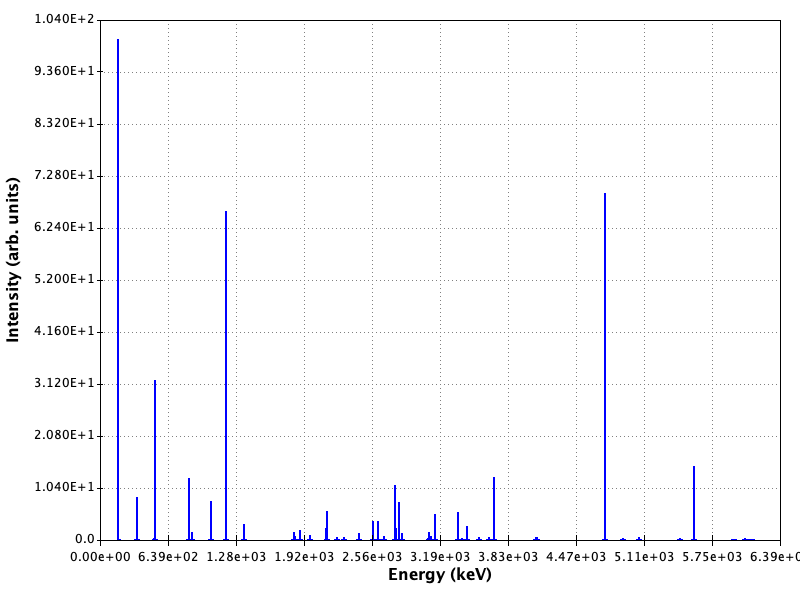
\includegraphics[width=\linewidth]{graphics/thermalgammaspectrum.png}
    \caption{Thermal Neutron Capture Gammas for an $\ce{^{40}Ar}$ target. Strongest transition: $E(\gamma) = 167.30 \pm 0.2$ (keV), $I(\gamma) = 74.028 \pm N/A$ (keV).  Thermal Neutron Capture Cross Section (2006MuZX): $0.66 \pm 0.01$ (b).  Results taken from \href{https://www.nndc.bnl.gov/capgam/byTarget/z018_40Ar.html}{NNDC} \cite{NNDC}.}
    \label{fig:my_label}
\end{figure}

\begin{table}[H]
    \centering
    \begin{tabular}{|c|c|c|c|c|c|}
        \hline
        $E_{\gamma}$ & $I_{\gamma}$ & $E_i(\mathrm{level})$ & $J_i^{\pi}$ & $E_f$ & $J_f^{\pi}$\\
        \hline
        \hline
        167.3(2) & 79.6 & 167.3 & $5/2^-$ & 0 & $7/2^{-}$\\
        \hline 
    \end{tabular}
    \caption{Gamma cascade statistics...}
    \label{tab:my_label}
\end{table}

\begin{figure}[H]
    \centering
    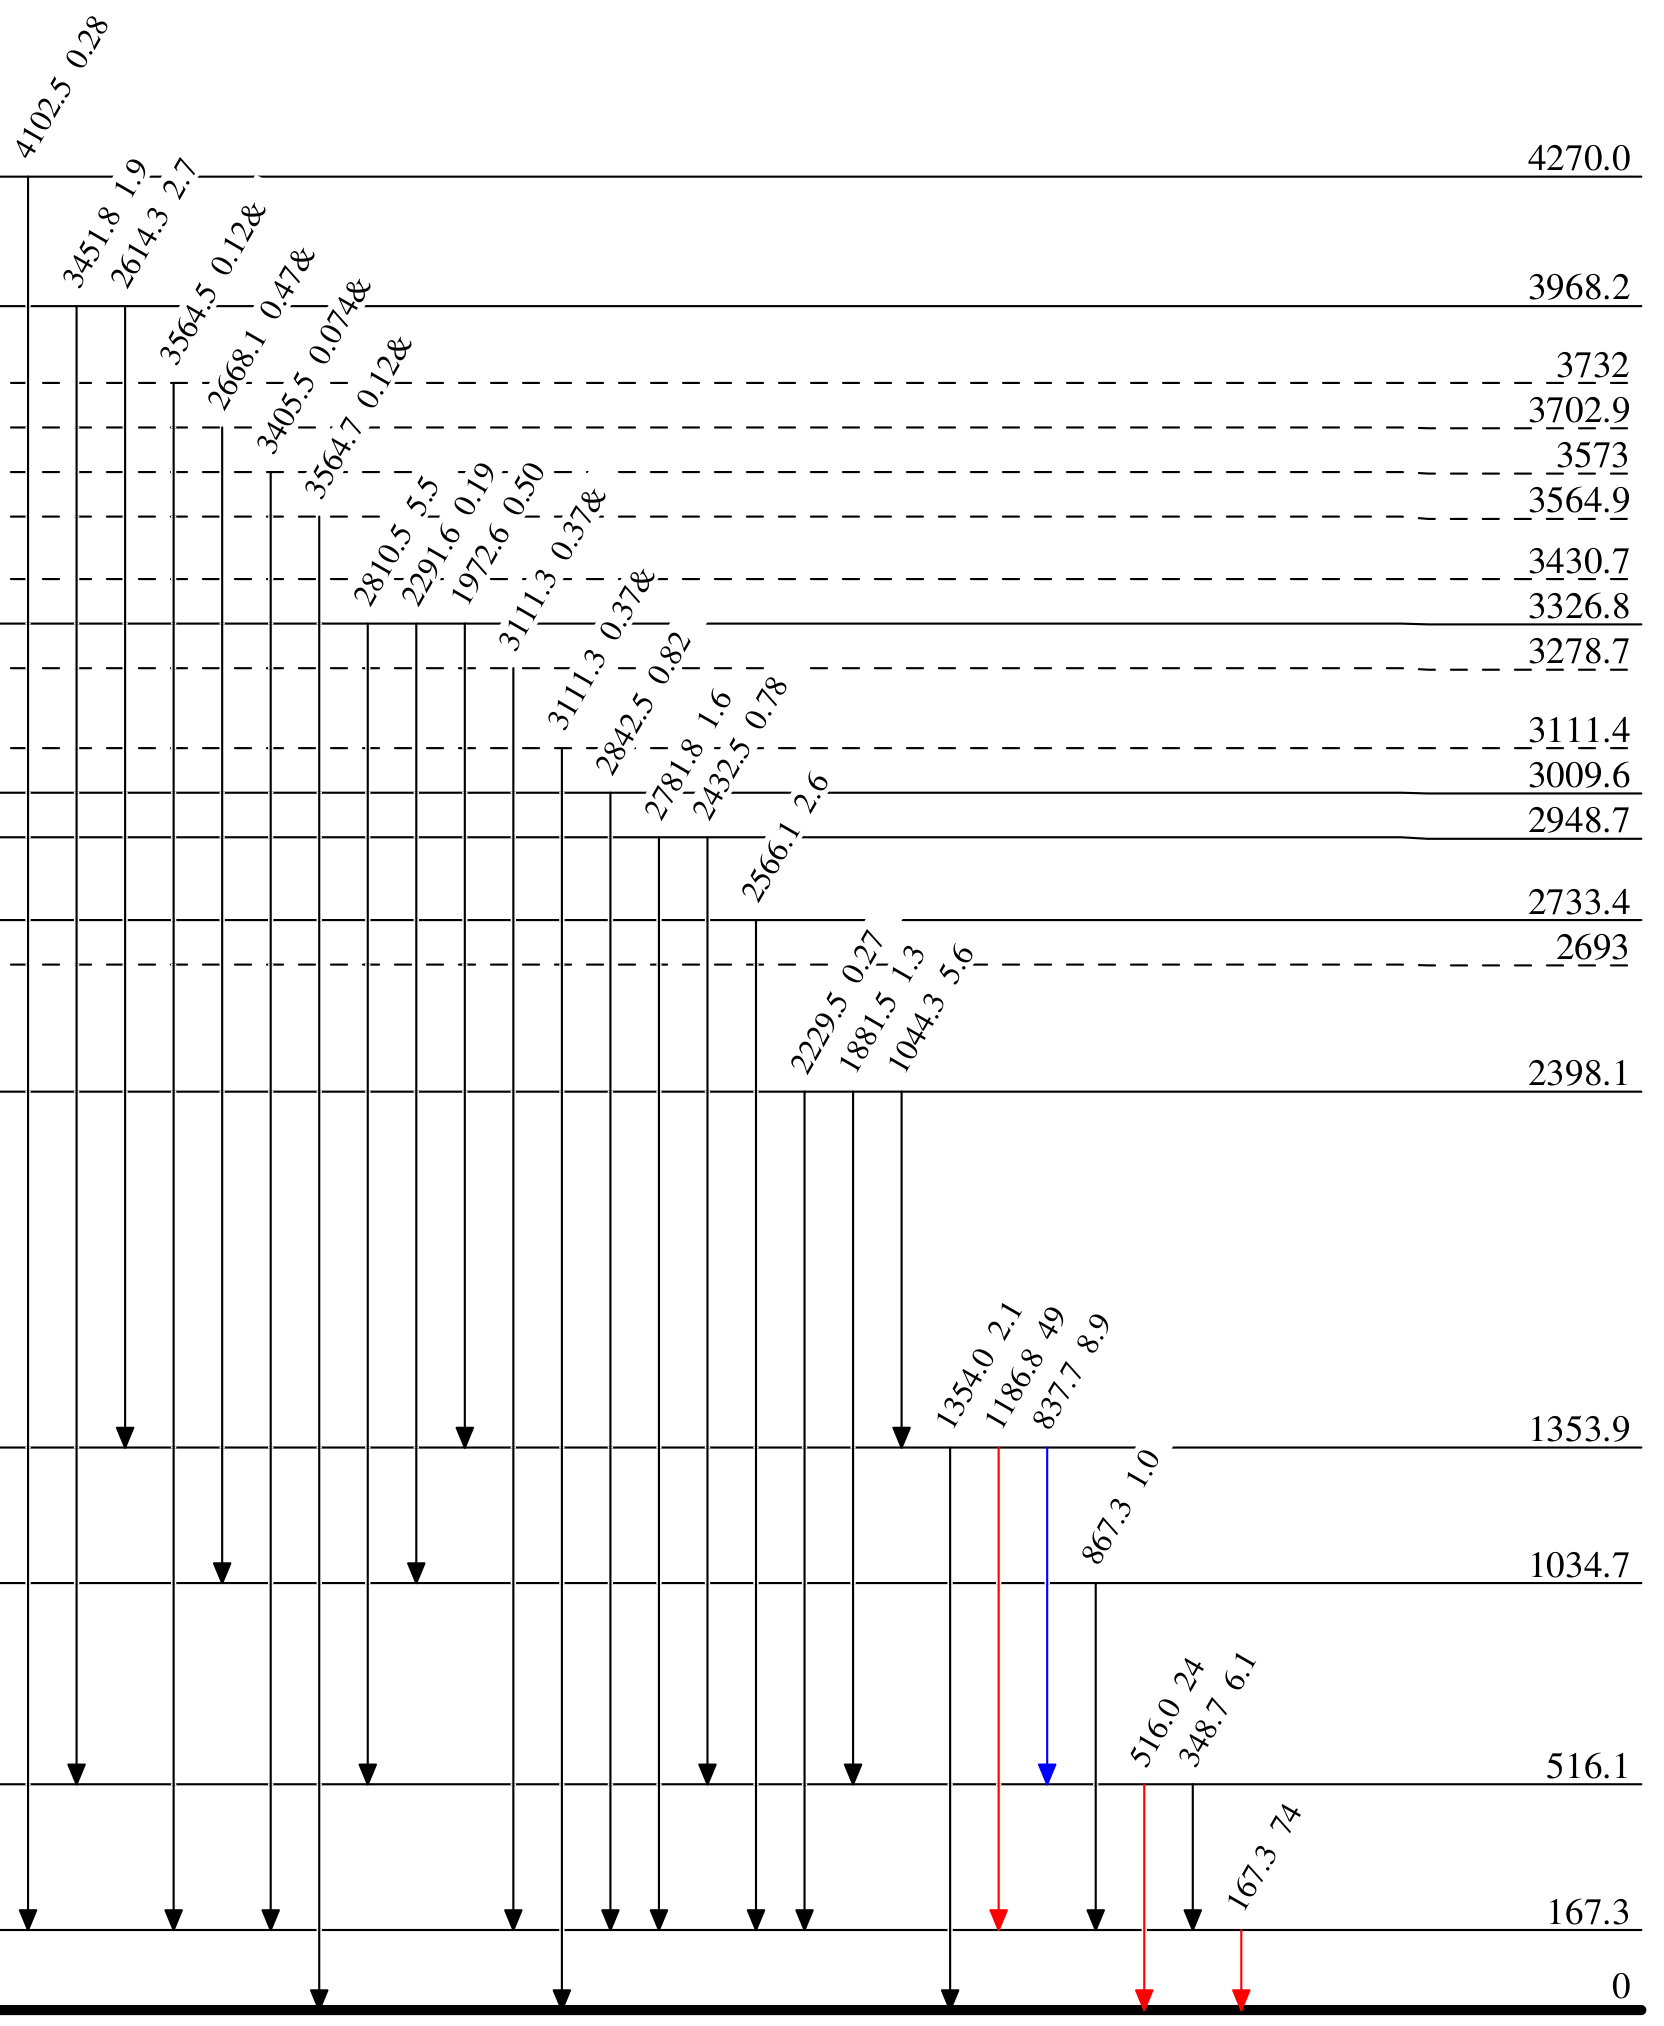
\includegraphics[width=\linewidth]{graphics/gamma_cascade_secondary.png}
    \caption{Emission diagram containing secondary gamma emissions from neutron capture on $\ce{^{40}Ar}$.}
    \label{fig:my_label}
\end{figure}

\index{Internal Conversion}\subsubsection{Internal Conversion}

\subsection{Ionization and Scintillation}


\subsection{Electron Drift and Recombination}

\newpage

\section{Computing Environment Setup}
There are several pieces of infrastructure that we will discuss in this section including how to set up the computing environment necessary to conduct the neutron calibration simulation and analysis.  This will require the following:
\begin{enumerate}
    \item \hyperref[fnalcomputing]{FNAL computing account} - most of the simulation will be carried out on FNAL machines.
    \item \hyperref[kerberos]{kerberos} - you will need a valid kerberos ticket to access your FNAL account.
    \item \hyperref[larsoftsetup]{LArSoft} - some familiarity with LArSoft will be required.
    \item \hyperref[eventdisplays]{event displays} - some familiarty with event display technology is encouraged.
    \item \hyperref[slaccomputing]{SLAC computing account} - the machine learning pipeline requires a SLAC computing account.
\end{enumerate}

\subsection{FNAL Computing Accounts}\label{fnalcomputing}
In order to conduct the neutron calibration study, we will make use of several computing systems.  The first one we will utilize is the \href{https://computing.fnal.gov/neutrino-muon-physics-computing/}{Fermilab computing cluster} that is dedicated to neutrino physics.  One will need to set up the appropriate accounts, which you can do by following the introduction in the DUNE computing tutorial from May 2021 \cite{DUNEComputing2021}\footnote{See the instructions here: \url{https://dune.github.io/computing-training-202105/setup.html}.}.  We will follow closely the instructions written in the tutorial \cite{DUNEComputing2021}.

\index{kerberos}\marginlabel{
\includegraphics[width=.4\linewidth]{graphics/dog-ring.jpg} kerberos:}\label{kerberos}
You will need a valid kerberos account \cite{kerberos} in order to log into the FNAL computing system.  Once you have an account set up, you will first have to edit the configuration file stored in
\begin{code}{text}
/etc/krb5.conf
\end{code}
As discussed in \cite{DUNEComputing2021}, you can find a few templates for FNAL \href{https://authentication.fnal.gov/krb5conf/}{here} for macOS, Windows and Linux -- there are both scientific Linux (SL7) and CentOS versions.  As mentioned in the tutorial \cite{DUNEComputing2021}, more information on the configuration file can be found \href{https://fermi.servicenowservices.com/kb_view.do?sysparm_article=KB0011315}{here}.  In order to login to an FNAL account, you will need an active kerberos \textit{ticket}, which will be valid for 26 hours once it is generated.  From a local machine, you can issue the following command to generate a ticket:
\begin{code}{shell}
kinit
\end{code}
or a more verbose version:
\begin{code}{shell}
kinit -f <username>@FNAL.GOV
\end{code}
where the ``-f'' option means that the ticket is forwardable to other machines.  This will then ask for your kerberos password,
\begin{code}{text}
Password for <username>@FNAL.GOV
\end{code}
You can use the ``klist'' command to see which tickets are active on your machine.  An example is the following:
\begin{code}{text}
Ticket cache: FILE:/tmp/krb5cc_1000
Default principal: ncarrara@FNAL.GOV

Valid starting       Expires              Service principal
10/03/2021 11:12:21  10/04/2021 13:12:15  krbtgt/FNAL.GOV@FNAL.GOV
	renew until 10/10/2021 11:12:15
\end{code}
A ticket will expire after 26 hours, and so a new one will need to be generated, however you can refresh a previous ticket for up to a week by issuing the following command:
\begin{code}{shell}
kinit -R
\end{code}
where ``-R'' requests a refresh on a previous ticket.

\index{dunegpvm}\marginlabel{Logging into dunegpvms:}One last step must be completed before login, which is to edit the secure shell configuration file
\begin{code}{text}
~/.ssh/config
\end{code}
If this file doesn't exist, then create it and fill it with the following minimal contents:
\begin{code}{shell}
Host *.fnal.gov
ForwardAgent yes
ForwardX11 yes
ForwardX11Trusted yes
GSSAPIAuthentication yes
GSSAPIDelegateCredentials yes
\end{code}
Once you have a valid kerberos ticket, you can log into a \textit{DUNE general purpose virtual machine} (dunegpvm) by issuing the command:
\begin{code}{shell}
ssh <username>@dunegpvmXX.fnal.gov
\end{code}
where ``XX'' is a number between 01 and 15 (i.e. there are 15 available dunegpvm login nodes to be utilized by the experiment).

\index{dunebuild}\marginlabel{dunebuild servers:}Whenever you want to compile something on the FNAL cluster, you should use a dunebuildXX server, rather than the general purpose machines.  The dunebuildXX servers are configured to have 16 available cores per node for compiling, so that compile jobs take less time than on a dunegpvmXX.  There are currently two dunebuildXX servers, dunebuild01 and dunebuild02.  Once one has a kerberos ticket, they can log in to one of these in the standard way,
\begin{code}{shell}
ssh <username>@dunebuildXX.fnal.gov
\end{code}


\subsection{LArSoft Environment Setup}\label{larsoftsetup}
Once one is able to log into one of the dungpvmXXs, the next step is to set up the proper environment for running jobs and conducting simulation and reconstruction.  In most cases, one will need to first run the DUNE setup script, which is located in,
\begin{code}{text}
/cvmfs/dune.opensciencegrid.org/products/dune/
\end{code}
The script ``setup\_dune.sh'' should be sourced,
\begin{code}{shell}
source /cvmfs/dune.opensciencegrid.org/products/dune/setup_dune.sh
\end{code}
which should show the following output:
\begin{code}{text}
Setting up larsoft UPS area... /cvmfs/larsoft.opensciencegrid.org/products/
Setting up DUNE UPS area... /cvmfs/dune.opensciencegrid.org/products/dune/
\end{code}

\index{ups}\marginlabel{unix product support (UPS):}This sets up the LArSoft and DUNE UPS environments.  UPS, or \href{https://mu2ewiki.fnal.gov/wiki/UPS}{\textit{Unix Product Support}}, is a tool developed by Fermilab that controls ``external'' unix programs on the FNAL cluster.  This includes things like \href{https://art.fnal.gov/}{\textit{art}} \cite{art}, \href{https://geant4.web.cern.ch/}{Geant4} \cite{geant4_1,geant4_2,geant4_3}, \href{https://larsoft.org/}{LArSoft} \cite{larsoft}, etc.  To see what commands are available from UPS see the \hyperref[appendixups]{appendix}.  To list the available products in our session we can invoke the command:
\begin{code}{shell}
ups list -aK+
\end{code}
which will print out a pretty extensive list.  To narrow in on a particular product, one could try adding something like
\begin{code}{shell}
ups list -aK+ geant4
\end{code}
which will list all of the available Geant4 implementations.  Each product contains information about what kind of compiler was used,
\begin{code}{text}
"geant4" "v4_10_6_p01d" "Linux64bit+3.10-2.17" "c7:prof" "" 
"geant4" "v4_10_6_p01d" "Linux64bit+3.10-2.17" "e20:prof" "" 
"geant4" "v4_10_6_p01d" "Linux64bit+3.10-2.17" "debug:e20" "" 
"geant4" "v4_10_6_p01d" "Linux64bit+3.10-2.17" "c7:debug" "" 
\end{code}
We can see in this above list of Geant4 implementations a set of ``prof'', or \textit{professional} installations, as well as two ``debug'' ones, which each have a ``e20'', or \textit{c++20}, and a ``c7'', or \textit{clang7}, version.  For more information on UPS see \href{https://mu2ewiki.fnal.gov/wiki/UPS}{this site}, or the \href{https://citeseerx.ist.psu.edu/viewdoc/download?doi=10.1.1.199.4454&rep=rep1&type=pdf}{UPS/UPD manual}.

\index{dunetpc}\marginlabel{
\includegraphics[width=.4\linewidth]{graphics/neutrino.png} dunetpc:} For simulation and some reconstruction purposes, we will need to set up our environment with a version of the \href{https://github.com/DUNE/dunetpc}{dunetpc} software, which uses several modules from the LArSoft framework.  This can be done by using the ``setup'' command from UPS by specifying which version you want to use.  For this study, we will use ``v09\_31\_00'' with the qualifiers ``e20:prof''.  We can set up dunetpc with the following command:
\begin{code}{shell}
setup dunetpc v09_31_00 -q e20:prof
\end{code}
where ``-q'' comes before the qualifiers.  The setup command will generate a set of environment variables that will point to the version we have chosen.  

\paragraph{Building a local LArSoft of DUNETPC ---}If you want to build your own local copy of LArSoft, or dunetpc, the following set of steps will give you a fresh installation.  The setup uses \textit{ninja} which makes recompiling very quick, which will be extremely useful when writing custom modules that require small changes and frequent recompiling.
\begin{code}{shell}
source /cvmfs/dune.opensciencegrid.org/products/dune/setup_dune.sh
#you'll need to match the larsoft version with the latest dunetpc version
setup larsoft <version> -q <quals> 
setup ninja
# create the directory where you want your local build
mkdir <custom_larsoft_directory>
cd <custom_larsoft_directory>
# generate a new development folder structure
mrb newDev        
# set up environment variables
source localProducts*/setup
cd srcs
# download the corresponding dunetpc software
mrb g dunetpc
cd $MRB_BUILDDIR
# set up the build
mrbsetenv
# build using 32 cores and ninja
mrb install -j 32 --generator ninja
\end{code}
Once this environment has built successfully and one wished to recompile after small changes, then simply enter the command:
\begin{code}{shell}
ninja -C $MRB_BUILDDIR -j 32 install
\end{code}
If you log out of your current dunebuildXX, or something got messed up with the environment variables, then on a subsequent login you will first need to issue the commands
\begin{code}{shell}
source /cvmfs/dune.opensciencegrid.org/products/dune/setup_dune.sh
setup larsoft <version> -q <quals> 
setup ninja
cd <custom_larsoft_directory>
source localProducts*/setup
\end{code}




\subsection{Fermilab Hierarchical Configuration Language (FHiCL)}All software which uses the \textit{art} event processing framework \cite{art}, must specify jobs using the \textit{Fermilab Hierarchical Configuartion Language} (FHiCL) -- pronounced ``fickle'' -- as a configuration language \cite{FHiCL}\footnote{A quick start guide for FHiCL can be found \href{https://cdcvs.fnal.gov/redmine/documents/327}{here}.}


\index{FHiCL!services}\marginlabel{services:}

\index{FHiCL!source}\marginlabel{source:}

\index{FHiCL!physics}\marginlabel{physics:}

\index{FHiCL!physics!producers}\marginlabel{producers:}

\index{FHiCL!physics!filters}\marginlabel{filters:}

\index{FHiCL!physics!analyzers}\marginlabel{analyzers:}

\index{FHiCL!outputs}\marginlabel{outputs:}

\index{FHiCL!trigger\_paths}\marginlabel{trigger\_paths:} A trigger path is a configured sequence of module labels, each of which correspond to either a \textit{producer} or a \textit{filter} (i.e. a module which modifies events).

\index{FHiCL!end\_paths}\marginlabel{end\_paths:} Like a trigger path, an end path is a configured sequence of modules labels, each of which corresponds to an \textit{analyzer} or \textit{output} module (i.e. modules which cannot modify events).


\subsection{Event Displays}\label{eventdisplays}
This section will cover the basics of various event display technologies including the canonical event display from LArSoft, as well as \hyperref[webevd]{webevd} and the displays available in the wire-cell toolkit.

\index{vncserver}\marginlabel{
\includegraphics[width=.4\linewidth]{graphics/remmina.png} VNC Viewer:}
One crucial piece of technology will be to use a \textit{VNC connection} to the DUNE virtual machines that will allow the user to access a remote desktop.  This is crucial if one wants to use the canonical event display or other programs on the cluster that generate plots or images.  A tutorial for setting up the appropriate environment for the SBN experiment, written by Dominic Brailsford, can be found \href{https://sbnsoftware.github.io/sbndcode_wiki/Viewing_events_remotely_with_VNC.html}{here}, however we will reiterate the instructions below.  As explained in the tutorial, you must do three things:
\begin{enumerate}
    \item Pick a number between 0 and 99 for your VNC connection.
    \item Choose the dunegpvmXX that you want to use for your VNC connection (where again, XX must be between 01 and 15).
    \item Download and install a VNC viewer that works on your platform (A good one for Linux is \href{https://remmina.org/}{Remmina} \cite{remmina}, however Macs already come with one installed).
\end{enumerate}
Going off of step 1 above, we first want to log in to any given dunegpvmXX and try the following command,
\begin{code}{shell}
vncserver :50 -localhost -bs
\end{code}
where I've used ``50'' as my chosen number.  The qualifier ``localhost'' must be included for this to work on FNAL servers and the ``bs'' qualifier ...  If the number you chose for your server is already taken, you'll see a message like
\begin{code}{text}
vncserver :50 already running (hopefully owned by you).  Not attempting to start the vncserver...
\end{code}
so, you will have to choose a different number and try again.  One can also specify a custom geometry for the output display by issuing the command:
\begin{code}{shell}
vncserver :50 -localhost -bs -geometry 1680x1500
\end{code}
Once you have picked a number that hasn't been taken, you need to edit ``\~/.bash\_profile'' so that it includes the following lines (replacing the ``VNCNUM=50'' with the number you choose (see the \href{https://sbnsoftware.github.io/sbndcode_wiki/Viewing_events_remotely_with_VNC.html}{tutorial} for a clean version to copy/paste from):
\begin{code}{bash}
#VNC stuff
VNCNUM=50 #CHANGE THIS NUMBER TO WHATEVER VNC SERVER NUMBER YOU PICKED
if [[ `hostname` == *"gpvm"* ]] #only start VNC servers on the gpvms (i.e. not on the build machines)
then
  export DISPLAY=localhost:$VNCNUM #Export the display to point to the VNC server
  if [ `lsof -i -P -n | grep $(expr 5900 + ${VNCNUM}) | wc -l` -eq 0 -o `lsof -i -P -n | grep $(expr 6000 + ${VNCNUM}) | wc -l` -eq 0 ]
  then
    echo "vncserver :$VNCNUM not running.  Starting now...." 
    vncserver :$VNCNUM -localhost -bs    #Check if the VNC server is running and start it if not (-localhost mandatory!)
  else
    echo "vncserver :$VNCNUM already running (hopefully owned by you).  Not attempting to start the vncserver..." 
  fi
fi
\end{code}
For the next step, we will follow a simpler path than one would normally take to complete the connection by creating a ssh login script in the ``\~/.ssh/config'' file.  If that file doesn't exist, although it should if you've followed the previous subsection, then create it and add the following lines:
\begin{code}{bash}
Host dunegpvmXX
  HostName dunegpvmXX.fnal.gov
  User <username>
  ForwardAgent yes
  ForwardX11 yes
  ForwardX11Trusted yes
  GSSAPIAuthentication yes
  GSSAPIDelegateCredentials yes
  LocalForward 5901 localhost:5950
\end{code}
The important part of this is the forwarding of ``localhost:5950'' to the local address of ``5901'', which is where you'll want to point the VNC viewer.

\index{evd}\marginlabel{evd:}The canonical event display can be run (once the appropriate setup of LArSoft products has been conducted) by issuing a command like:
\begin{code}{shell}
lar -c evd_dune.fcl <event_file.root>
\end{code}
where the ``event\_file.root'' is the root file containing the events.

\index{WebEVD}\marginlabel{WebEVD:}\label{webevd}Another useful tool, called \href{https://github.com/LArSoft/webevd}{WebEVD},  was developed by Chris Backhouse and is included as part of the LArSoft framework as a UPS product.  The current version as of writing these notes is ``v09\_06\_01'', which you can invoke by using the following command:
\begin{code}{shell}
setup webevd v09_06_01 -q e20:prof
\end{code}
Once the WebEVD is loaded, one can invoke it by using a command like:
\begin{code}{shell}
lar -c webevdjob_fd.fcl <file_to_display.root>
\end{code}
which will then give you instructions for how to view the file like the following:
\begin{code}{text}
First run
ssh -L 1075:localhost:1075 <username>@dunegpvmXX.fnal.gov

and then navigate to localhost:1075 in your favorite browser.
\end{code}

\index{bee-display}\marginlabel{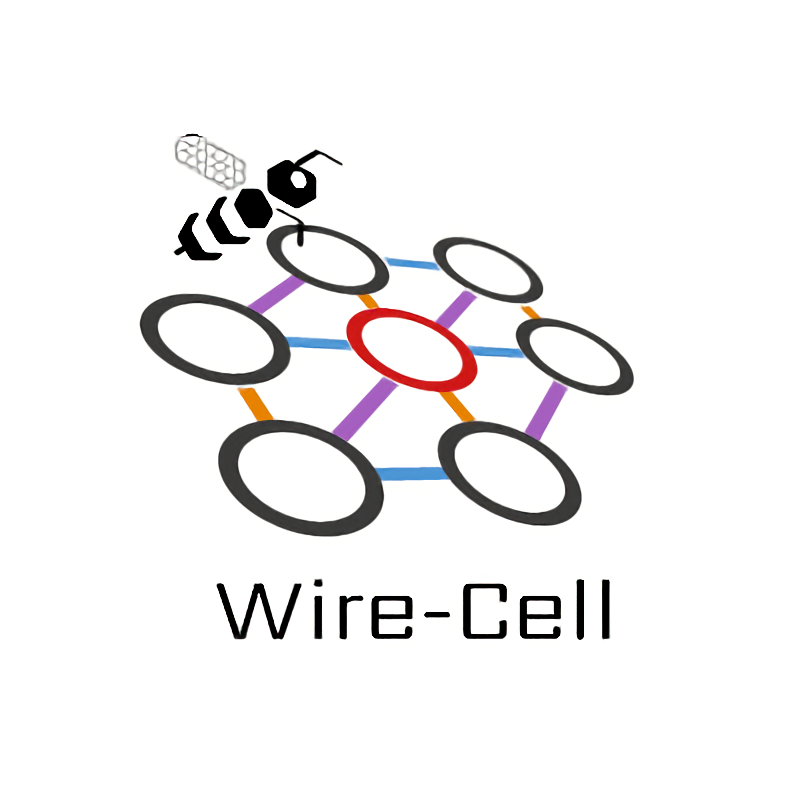
\includegraphics[width=.4\linewidth]{graphics/wire-cell-bee-400x400.png} wire-cell toolkit bee display:}
Another extremely useful set of tools comes from the \href{https://github.com/WireCell}{wire-cell toolkit} \cite{WCT}.


\subsection{SLAC Computing Accounts}\label{slaccomputing}
In order to run the machine learning parts of this analysis, you will need access to a decent GPU (at least if you are interested in actually running the training of models).  One of the main computational overheads comes from the amount of memory that the GrapPA network uses during training -- this step will fail on a GPU with only 8gb of RAM.


\index{SDF}\marginlabel{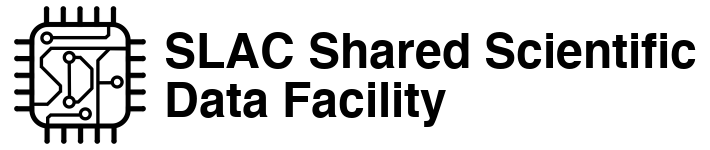
\includegraphics[width=\linewidth]{graphics/sdf-header.png}\\ SLAC shared scientific data facility (SDF):}  The SLAC shared scientific data facility (SDF) \cite{SDF} provides dedicated NVidia V100's and A100's for the DeepLearnPhysics group.  There are two ways to utilize this resource, either through the web (using a jupyter notebook or jupyter-lab setup) or through the terminal.  In either case, one will want to make use of the singularity images that the DLP group has pre-compiled for using their software.

In order to use SDF, you can either ssh in,
\begin{code}{shell}
ssh <username>@sdf.slac.stanford.edu
\end{code}
or you can use the API on the website, which is located \href{https://sdf.slac.stanford.edu/pun/sys/dashboard}{here}.
\index{SDF!singularity}

\index{singularity}\marginlabel{
\includegraphics[width=.4\linewidth]{graphics/singularity-logo.svg} singularity:} Singularity \cite{singularity,singularity-github} is a software library that manages containers, much like docker \cite{docker}, which consist of pre-configured development environments that can be swapped out on the fly.  In order to use singularity within the context of a terminal login, you must first get the image you want to work with:
\begin{code}{shell}
singularity pull <image>
\end{code}
For the DLP group, there are images kept in their respective \href{https://hub.docker.com/u/deeplearnphysics}{docker directory}.  One can look on their site to figure out the image one wants to use, for example:
\begin{code}{shell}
singularity pull docker://deeplearnphysics/larcv2:ub18.04-cuda10.2-pytorch1.7.1-edepsim
\end{code}
Make sure to not do this in your home directory, as it will generally be a very large file (several gigabytes).  Once a container is downloaded, you can run it by simply issuing the command:
\begin{code}{shell}
singularity exec --nv <image> bash
\end{code}
where the ``--nv'' command tells the system to connect the GPU interface and ``bash'' tells the system you want to run a bash session (this would get changed to jupyter if using the API).  Once you are inside the singularity environment, it will act like a virtual machine with a system of folder hierarchies.  In order to access folders outside of the image, you will have to \textit{bind} them when running the exec command:
\begin{code}{shell}
singularity exec --nv -B <folders_to_bind> <image> bash
\end{code}
For our purposes, it is common to bind the directories ``/sdf'', ``/scratch'', ``/lscratch'' and ``/gpfs'':
\begin{code}{shell}
singularity exec --nv -B /sdf,/scratch,/lscratch,/gpfs <image> bash
\end{code}
As a note, you must write the directories with no spaces in between the commas, otherwise singularity will fail to load the session.

\index{SDF!singularity}\marginlabel{API login:}Once logged in, you can start a new session by clicking on ``My Interactive Sessions'' in the top margin of the page, and then click on ``Jupyter'' in the ``Services'' list.  This will bring up a configuration with the following fields:
\begin{table}[H]
\centering
\begin{tabular}{|p{0.24\linewidth}|p{0.71\linewidth}|}
    \hline
     Field & Example\\
     \hline
     \hline
     Jupyter Instance & neutrino-jupyter/latest\\
     \hline
     Commands to initiate Jupyter & \makecell[l]{export SINGULARITY\_IMAGE\_PATH\\
                                                 =/sdf/group/neutrino/images/latest.sif\\ 
                                                 export PYTHONPATH=""\\
                                                 function jupyter() \{ singularity exec --nv -B\\
                                                 /sdf,/scratch,/lscratch\\
                                                 \$\{SINGULARITY\_IMAGE\_PATH\} jupyter \$\@; \}}\\
     \hline
     \textit{Use JupyterLab instead of Jupyter Notebook?} & Yes\\
     \hline
     \textit{Disable JupyterLab extensions (Run with --core-mode)} & No\\
     \hline
     Partition & neutrino\\
     \hline
     Number of hours & 24\\
     \hline
     Number of CPU cores & 4\\
     \hline
     Total Memory to allocate & 20096\\
     \hline
     Number of GPUs & 1 \\
     \hline
     GPU Type & Nvidia Tesla A100\\
     \hline
\end{tabular}
\caption{Set of configuration values for spinning up an SDF GPU session with a Jupyter environment.}
\end{table}
As of writing these notes there are currently 16 Ampere (A100) architecture GPUs and 10 Volta (V100) architecture GPUs available for use by the DLP team.




\index{Deep Learn Physics}\subsection{DeepLearnPhysics}
\href{https://deeplearnphysics.org/}{DeepLearnPhysics} (DLP) \cite{DLP1,DLP2,DLP3} is a group that originated at SLAC consisting of scientists, post-docs and graduate students working on various LArTPC experiments such as MicroBooNE, SBND, ICARUS and DUNE.  The group is interested in developing machine learning techniques for reconstruction and analysis of LArTPC data.

Of course the main goal of many of these experiments is to extract information about neutrino interactions, such as their interaction energy, but this requires us to first be able to identify such reactions.  Due to the design of the experiments, the data is inherently three($+n$)-dimensional -- events are described by collections of energy (and charge) depositions in three-dimensional space.  The goal of the DLP reconstruction effort is to construct a series of \textit{hierarchical features} from the $(3+n)$-dimensional input data.  This includes high level features such as track and shower identification/reconstruction, interaction identification, energy and momentum, but also low level features such as pixel level segmentation and tagging points of interest like vertices and track beginning and ending points.  Each step in the reconstruction chain can be broken down into the following generic hierarchy:
\begin{enumerate}
    \item \textbf{Pixel level semantics} - Pixel feature extraction and points of interest identification.  Here we want to aggregate local information to assign to each pixel a set of labels (such as \texit{track}, \texit{shower}, \textit{Michel electron}, etc.) as well as identify key points of interest (such as start and end points of tracks/showers and interaction vertices). 
    \item \textbf{Particle clustering} - Clustering of pixels of similar semantic type into clusters (or fragments) using canonical clustering techniques together with graph neural network approaches.
    \item \textbf{Particle type and energy/momentum reconstruction} - Identifying particles which generated the charge depositions (such as muons, pions, protons, neutrons, etc.) as well as their energy/momentum by using information from the previous steps.
    \item \textbf{Interaction (particle flow) reconstruction} - Inference of various interactions within an event using the information determined from the previous steps.
\end{enumerate}
Applying machine learning to solve each of these steps has several benefits.  First, it allows us to compile the entire reconstruction chain into a single optimization problem, i.e. by chaining together each of the steps above, we can optimize the entire sequence together.  In addition, it allows us to construct a model agnostic approach to reconstruction, since the model can be applied easily to events it has never seen and still produce some reconstructed output.  An overview of the DLP model is shown below:

\begin{figure}[H]
    \centering
    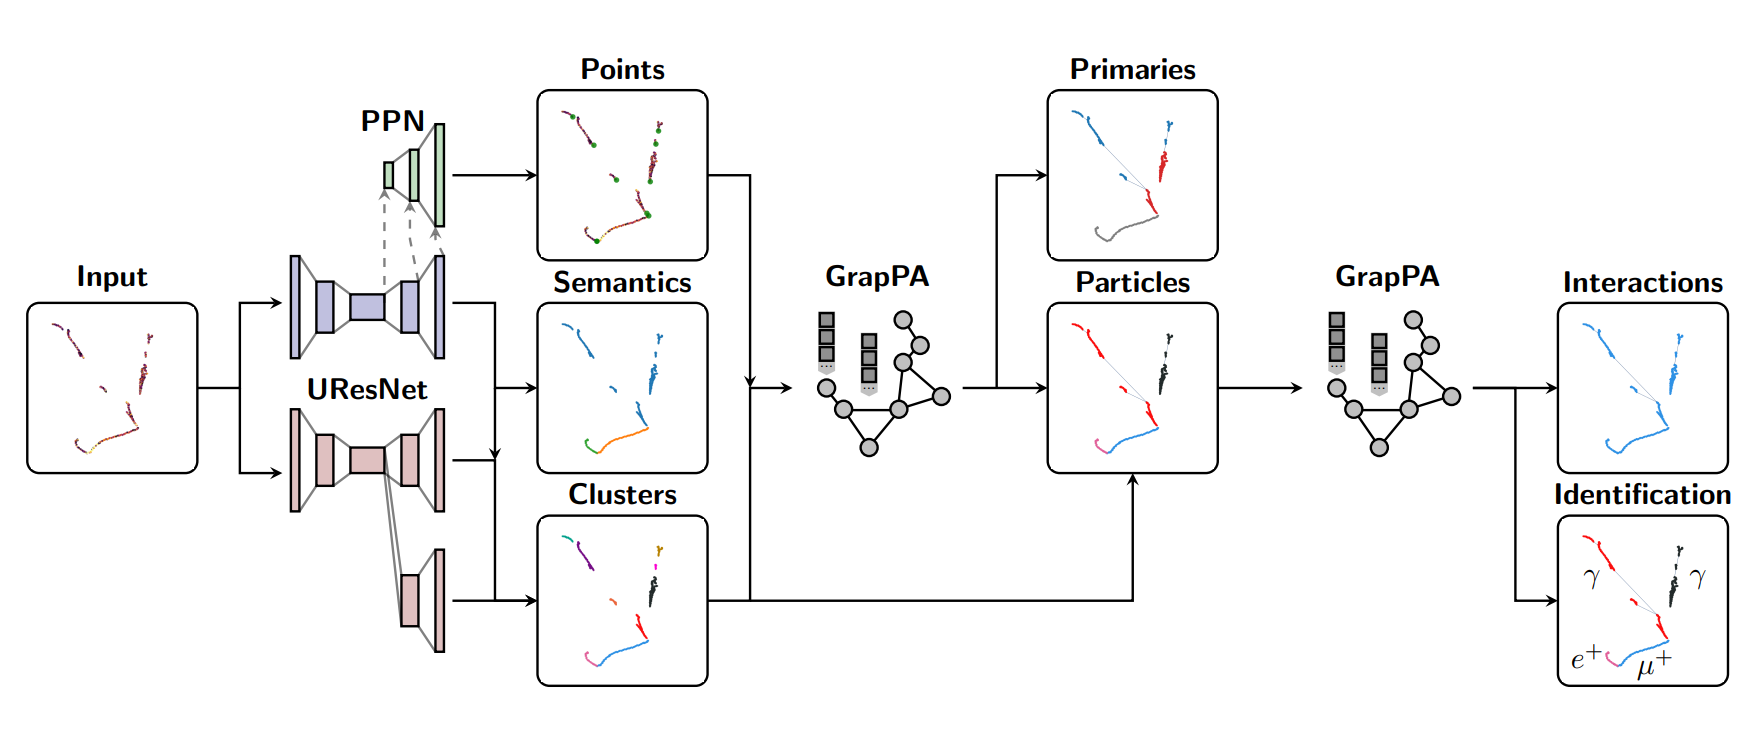
\includegraphics[width=\linewidth]{graphics/full_chain.png}
    \caption{Schematic of the full reconstruction chain for LArTPC MLReco3D.}
    \label{full_chain}
\end{figure}

\index{PILArNet}\marginlabel{PILArNet:} The DLP group has constructed a public dataset called PILArNet \cite{PILArNet} (or \textit{Particle Imaging Liquid Argon Net}) for benchmarking their model.  The data consists of 300,000 events...

\subsubsection{LArTPC\_MLReco3D}

\index{mlreco3d!Semantic Segmentation!UResNet}\index{UResNet}\subsubsection{Sparse-UResNet}\label{uresnet}
For the semantic segmentation part of the network, mlreco3d utilizes the UResNet architecture \cite{UResNet,UNet}, which is a combination of the U-Net \cite{UNet} and ResNet (or ResidualNet) \cite{ResNet} architectures.  In addition, because the images are generally sparse in terms of active voxels, the segmentation step uses approaches developed for sparse image classification.  As of the time of writing this, the current mlreco3d semantic segmentation incorporates the \href{https://github.com/facebookresearch/SparseConvNet}{SparseConvNet} design \cite{SparseConvNet1, SparseConvNet2,Graham} to deal with the sparseness of the input data, however future iterations of the model are slated to use the \href{https://github.com/NVIDIA/MinkowskiEngine}{Minkowski Engine} \cite{MinkowskiEngine}.

\index{Sparse Tensor}\marginlabel{Sparse Tensors:}One of the key features of LArTPC data, is that geometrical representations tend to be sparse, in that most of the space in which the events live is empty.  This can be a problem for traditional neural networks, such as a vanilla convolutional network -- these types of geometrical representations are better suited for sparse networks.  Sparse convolution networks operate on \textit{sparse tensors}, which can be introduced in two different ways, either by making the matrix of weights sparse themselves, or by making the inputs sparse.  

Sparse images can be stored in a \textit{coordinate list representation}, which involves assigning to each non-zero element of the image a coordinate, and the value of the image at that coordinate.  This substantially reduces memory demands for sparse data.  In higher dimensions this is sometimes referred to as a \textit{High-dimensional COOrdinate list}, or (Hi-COO) representation.  The pixels, or voxels in higher dimensions, which are non zero in an input are called \textit{active input sites} and their values are stored in a list $\vec{\mathbf{f}}$, whereas the corresponding coordinates are stored in a separate list $\vec{\mathbf{c}}$.

The paper by Graham \cite{Graham} defines a sparse convolution in which each kernel region that contains an active input site gets updated to a new value through the convolution, even those sites which have input values of zero.  This causes a \textit{dilation} of the input space which is not necessarily desirable.  In order to retain the sparse nature of the input, Graham, Engelcke and Van Der Maaten define a \textit{submanifold sparse convolution} in \cite{SparseConvNet1} in which only active sites are convolved and active sites with zeros remain zero.  We can define a submanifold sparse convolution over a sparse tensor in the following way by constructing what's called a \textit{rulebook} \cite{SparseConvNet1}.  These rulebooks are constructed from hash tables that store the coordinates of all the active input sites.

\begin{figure}[H]
    \centering
    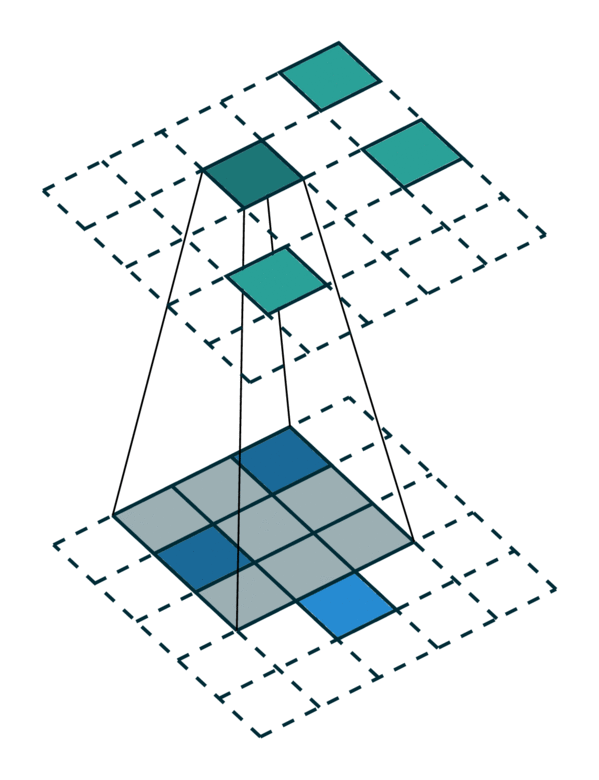
\includegraphics[width=.49\linewidth]{graphics/conv_sparse (1).png}
    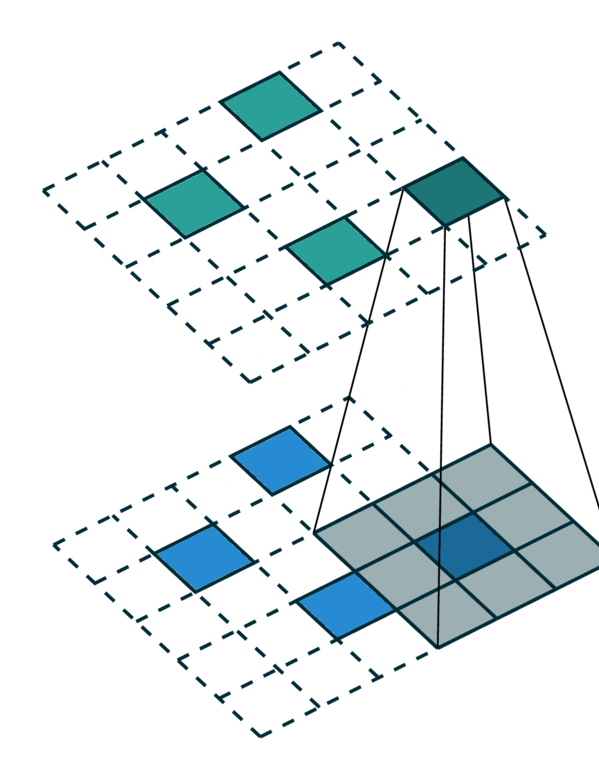
\includegraphics[width=.49\linewidth]{graphics/conv_sparse_conv.png}
    \caption{Examples of a sparse convolution (left) \cite{Graham} and a submanifold sparse convolution (right) \cite{SparseConvNet1}.  Figures taken from \href{https://nvidia.github.io/MinkowskiEngine/sparse_tensor_network.html}{here}.}
    \label{fig:my_label}
\end{figure}


\index{UNet}\marginlabel{UNet:}

\begin{figure}[H]
    \centering
    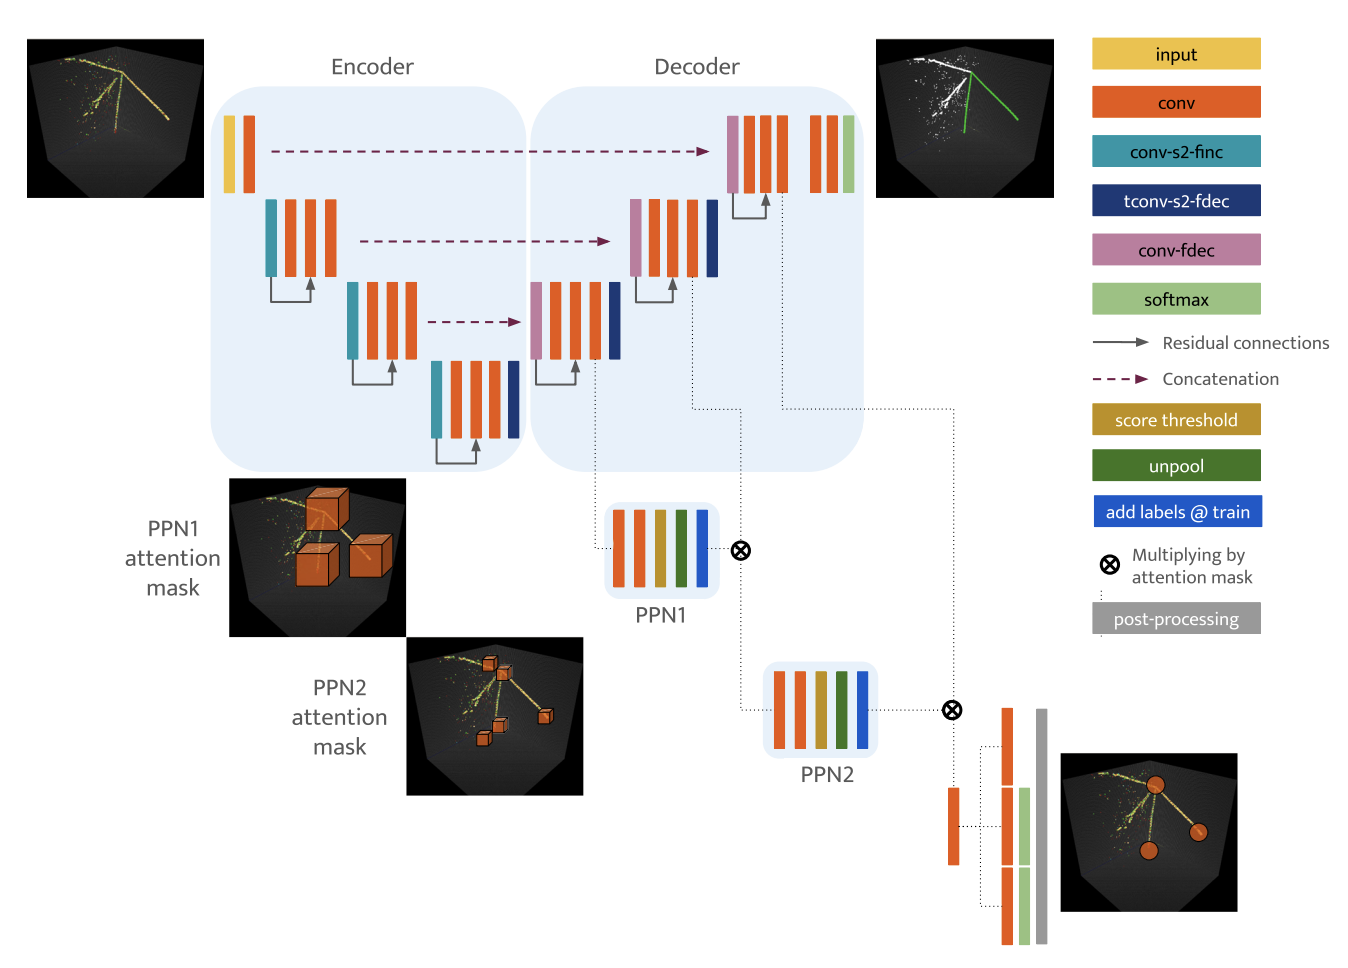
\includegraphics[width=\linewidth]{graphics/uresnet.png}
    \caption{Architecture of the Sparse-UResNet semantic segmentation network.  Image taken from \cite{DLP1}.}
    \label{fig:my_label}
\end{figure}

\marginlabel{
\includegraphics[width=.4\linewidth]{graphics/kazu_zoom.png}\\current difficulties with shower fragment parameters:}According to Francois Drielsma's \href{https://indico.fnal.gov/event/50338/contributions/225763/attachments/148106/190135/Recording_day2_morning.mp4}{tutorial}, currently, due to the lack of full detector simulations, shower fragments which are less than ten voxels in size are classified as low energy scatters, and are not considered as part of the fragment aggregation step.  The idea is that this should emulate some level of the reconstruction inefficiency due to the resolution of the detector, since most of the clusters with less than ten voxels are in the MeV to sub MeV range.  This cut will have to be adjusted as detector simulations improve.  This generates a shift in the reconstructed energy of showers by about 17\%, something which must be addressed in the future.  To correct the shift, one can either rely on the simulation to introduce a fudge factor (which is not preferred), or one can utilize standard candles such as Michel electrons for low energy or $\pi^0$ for high energy scatters.

\index{mlreco3d!Point Proposal Network}\index{Point Proposal Network}\subsubsection{Point Proposal Network}\label{pointproposalnetwork} In step with the semantic segmentation, the DLP model implements a point proposal network (PPN) \cite{DLP1} which attempts to label individual pixels as being of a certain type, such as the start and end of tracks or interaction vertices.  This is typically done in two steps, one at a lower resolution in which regions of interest are tagged, and then an additional step which attempts to narrow down the regions of interest to individual pixels.  A final step then classifies the points into different types.  

The PPN acts as a \textit{parasitic} network with respect to the Sparse-UResNet in that it influences the training of the weights for the semantic segmentation step.  

\index{SPICE}\subsubsection{SPICE}\label{SPICE}

\index{DBSCAN}\subsubsection{DBSCAN}\label{dbscan}
DBSCAN is a density based clustering algorithm \cite{DBSCAN1,DBSCAN2} which was first developed in 1996 and is still used widely today.  It is integrated as part of the standard reconstruction chain as well as in the mlreco3d framework.  Here we will attempt to give a brief explanation for how it works.

\index{mlreco3d!track!clustering}\subsubsection{Track Clustering}\label{trackclustering}
The clustering of voxels into tracks uses a density based approach called \hyperref[dbscan]{DBSCAN} \cite{DBSCAN1, DBSCAN2}, which groups nearby voxels into the same cluster based on the surrounding density of the points.  One issue with this approach is the fact that tracks that share a common vertex (called \textit{knots}) will be grouped together.  In order to get around this problem, we can use the results from the point proposal network to remove common vertex points from the DBSCAN step, and the algorithm does this by applying a mask to the input of the DBSCAN algorithm.

The track clustering step can be summarized as follows:
\begin{enumerate}
    \item Run \hyperref[dbscan]{DBSCAN} on the track voxels, which produces individual tracks (isolated) and groups of tracks which touch each other.
    \item Use the point predictions from the PPN to find knots (points shared by multiple tracks).
    \item Mask a sphere around each knot and run the \hyperref[dbscan]{DBSCAN} algorithm again.
    \item Associate remaining points with closest track instance (aggregation).
\end{enumerate}

Predicted track fragments are stored in the \hyperref[trackfragments]{`track\_fragments'} product.  


\index{mlreco3d!shower!clustering}\subsubsection{Shower Clustering}
Much like in \hyperref[trackclustering]{track clustering}, the clustering of showers is done in several steps:
\begin{enumerate}
    \item First, shower voxels are identified by the semantic segmentation part of the model (\hyperref[uresnet]{UResNet}).
    \item Next, \hyperref[dbscan]{DBSCAN} is used to cluster showers into fragments.
    \item Finally, shower fragments are aggregated with the \hyperref[grappa]{GrapPA} network.
\end{enumerate}


\index{mlreco3d!particle}\subsubsection{Particles}


\index{mlreco3d!clustering!performance}\subsubsection{Clustering Performance}
The various graph neural networks employed in mlreco3d use a set of different metrics to evaluate the network's performance.  As of writing these consist of:
\begin{itemize}
    \item \textbf{Purity} - the fraction of voxels in a predicted cluster which belong to a single true cluster - i.e. high purity means low over-clustering (mlreco3d implementation is in \href{https://github.com/DeepLearnPhysics/lartpc_mlreco3d/blob/develop/mlreco/utils/metrics.py}{mlreco/utils/metrics.py}).
    \item \textbf{Efficiency} - the fraction of the voxels in a true cluster which belong to a single predicted cluster - i.e. high efficiency means low under-clustering (mlreco3d implementation is in \href{https://github.com/DeepLearnPhysics/lartpc_mlreco3d/blob/develop/mlreco/utils/metrics.py}{mlreco/utils/metrics.py}).
    \item \textbf{Adjusted Rand Index (ARI)} - the fraction of voxel pairs which are either placed together or separated when they should(n't) be (mlreco3d implementation uses \href{https://scikit-learn.org/stable/modules/generated/sklearn.metrics.adjusted_rand_score.html#sklearn.metrics.adjusted_rand_score}{sklearn.metrics.adjusted\_rand\_score} from scikit-learn).
\end{itemize}
\index{Adjusted Rand Index}\index{mlreco3d!metrics!Adjusted Rand Index}\marginlabel{Adjusted Rand Index:}The ARI is an adjustment of the \textit{Rand Index} metric \cite{Rand}, which is the ratio of the number of pairs of points in a cluster which belong to the same true cluster ($X_{\mathrm{true}}$) and the total number of pairs of points in the predicted cluster,
\begin{equation}
    RI \stackrel{\mathrm{def}}{=} \frac{\sum_{i=1,j > i}^N\mathbbm{1}[(x_i,x_j) \in X_{\mathrm{true}}]}{\begin{pmatrix}N\\2\end{pmatrix}}.
\end{equation}
Essentially, it is the frequency of occurrence that any two points from a predicted cluster, are actually in the same true cluster.  The \textit{Adjusted Rand Index} \cite{ARI1} is supposed to be ``adjusted for chance,'' which means that it attempts to account for the fact that different clusterings may have different sizes, i.e. the Rand Index was built assuming that all cluster permutations happen with clusters of a fixed size, which is certainly not true in our case (e.g. one track may have thousands of voxels, while another may only have tens or hundreds).

To compute the ARI, one would typically first create a \textit{Contingency Table}, which looks like the following:
\begin{table}[H]
    \centering
    \begin{tabular}{c|c|c|c|c|c}
         $X/Y$ & $Y_1$ & $Y_2$ & $\cdots$ & $Y_s$ & sums\\
         \hline
         $X_1$ & $n_{11}$ & $n_{12}$ & $\cdots$ & $n_{1s}$ & $a_1$\\
         $X_2$ & $n_{21}$ & $n_{22}$ & $\cdots$ & $n_{2s}$ & $a_2$\\
         $\vdots$ & $\vdots$ & $\vdots$ & $\ddots$ & $\vdots$ & $\vdots$\\
         $X_r$ & $n_{r1}$ & $n_{r2}$ & $\cdots$ & $n_{rs}$ & $a_r$\\
         \hline
         sums & $b_1$ & $b_2$ & $\cdots$ & $b_s$ &\\
    \end{tabular}
    \caption{Contingency Table for two sets $X = \{X_1,\dots,X_r\}$ and $Y = \{Y_1,\dots,Y_s\}$.  For a clustering task, one typically has two sets of subsets of the data, $X_{\mathrm{true}}$ which contains the true clusters, and $X_{\mathrm{pred}}$ which contains the predicted clusters.  The numbers $n_{ij}$ are the number of elements in cluster $X_i$ which also appear in cluster $Y_j$.}
    \label{tab:my_label}
\end{table}
In the case of clustering, the two sets of subsets (clusters) of interest are $X_{\mathrm{true}}$, which contain the true clusters, and $X_{\mathrm{pred}}$ which contain the predicted clusters.  When two clusters within each set agree, the value of the number $n_{ii}$ will simply equal the number of elements in the cluster and all other values $n_{ij}$ should be zero for $j \neq i$ (provided the algorithm doesn't allow for overlap of clusters).  Thus, one should have (for perfect prediction), $n_{ii} = a_i = b_i$.  Once all the values of the matrix $n_{ij}$ are computed, one can evaluate the ARI metric, which is defined as,
\begin{equation}
    ARI \stackrel{\mathrm{def}}{=} \frac{RI - \langle RI\rangle}{\mathrm{max}(RI) - \langle RI\rangle} = \frac{\sum_{i,j}\begin{pmatrix}n_{ij}\\2\end{pmatrix} - \left[\frac{\sum_i\begin{pmatrix}a_i\\2\end{pmatrix}\sum_j\begin{pmatrix}b_j\\2\end{pmatrix}}{\begin{pmatrix}N \\ 2\end{pmatrix}}\right]}{\frac{1}{2}\left[\sum_i\begin{pmatrix}a_i\\2\end{pmatrix} + \sum_j\begin{pmatrix}b_j \\ 2 \end{pmatrix}\right]- \left[\frac{\sum_i\begin{pmatrix}a_i\\2\end{pmatrix}\sum_j\begin{pmatrix}b_j\\2\end{pmatrix}}{\begin{pmatrix}N\\2\end{pmatrix}}\right]},
\end{equation}





\index{GrapPA}\subsubsection{GrapPA}\label{grappa}


\index{GrapPA!metrics}\marginlabel{metrics:}


\index{mlreco3d!parsers}\subsubsection{Parsers}

\index{mlreco3d!products}\subsubsection{Products}

\begin{itemize}
    \index{mlreco3d!products!segment\_label}\item \textbf{segment\_label} - 
    \index{mlreco3d!products!particles\_label}\item \textbf{particles\_label} - 
    \index{mlreco3d!products!clusters\_label}\item \textbf{clusters\_label} - 
    \index{mlreco3d!products!segmentation}\item \textbf{segmentation} - A set of predictions for each label in the segmentation step of the network.  These currently include:
    \begin{enumerate}
        \item \textit{shower} - whether the energy deposition corresponds to a shower.  These events have a distinct topology from the other classes and are typically caused by either electrons, positrons or photons.
        \item \textit{track} - whether the energy deposition corresponds to a track.  Track topologies tend to be long one-dimensional objects (at least in an elementary sense).  Tracks could in principle by created by anything, but are typically caused by either \textit{heavy ionizing particles} (HIPs), such as protons, or \textit{minimal ionizing particles} (MIPs), such as muons or pions.
        \item \textit{michel} - whether the energy deposition corresponds to a Michel electron \cite{Michel}.  Michel electrons come from leptonic decays (specifically a muon or anti-muon) which produces the following channel for the muon:
        \begin{equation}
            \mu^{-} \rightarrow \nu_{\mu} + \bar{\nu}_e + e^-,
        \end{equation}
        or a similar channel for an anti-muon
        \begin{equation}
            \mu^+ \rightarrow \bar{\nu}_{\mu} + \nu_e + e^+.
        \end{equation}
        Michel introduced a parameter $\rho$ for characterizing the shape of the electron energy distribution coming from the decay of $\mu^-$.  Three more parameters were added to deal with the parity violating behavior of weak interactions, but all four parameters are referred to as ``Michel parameters''.  The values of the parameters $(\rho,\eta,\xi,\delta)$ are expected to have the values: $\rho=3/4$, $\eta=0$ and $\xi=\delta=1$.
        \item \textit{delta} - whether the energy deposition corresponds to a delta ray \cite{Delta}.  Delta rays are \textit{secondary} electrons that have enough energy to escape the primary interaction region and produce further ionization.  This further ionization is the main difference between inelastically scattered electrons and ones which are classified as delta rays.
        \item \textit{lescatter} - when the energy deposition corresponds to a low energy scatter (LES).  These are typically caused by photons which compton scatter off electrons and create an ionization ``blip''.  The source of the photons can range from nuclear processes, such as a capture, neutron-proton inelastic scatter, muon capture, intranuclear showers, etc., or they may come from electromagnetic showers.
    \end{enumerate}
    \index{mlreco3d!products!particles}\item \textbf{particles} - 
    \index{mlreco3d!products!track\_fragments}\item \textbf{track\_fragments}\label{trackfragments} - a collection of indices corresponding to a particular track fragment.  In general, `track\_fragments' will contain a list of arrays, each of which contains the voxel id's of the voxels that belong to a given fragment.
    \index{mlreco3d!products!particles\_asis}\item \textbf{particles\_asis}\label{particlesasis} - this product contains a set of truth information for each particle, such as:
    \begin{itemize}
        \item \textbf{id} - index of the particle in the list.
        \item \textbf{group id} - index of the group the particle belongs to (specifically a shower fragment attribute.  If a shower produces multiple fragments, then this references the parent fragment).
        \item \textbf{type} - PDG code.
        \item \textbf{momentum} - momentum of the particle ($MeV/c$).
        \item \textbf{energy} - total energy, including the particles mass ($MeV/c^2$).
        \item \textbf{visible fragment energy} - kinetic energy deposited in the volume for a specific fragment ($MeV/c^2$).
    \end{itemize}
    For a full list of attributes, see the \href{https://github.com/DeepLearnPhysics/larcv2/blob/develop/larcv/core/DataFormat/Particle.h}{Particle.h} file within the \href{https://github.com/DeepLearnPhysics/larcv2}{LArCV} package.
\end{itemize}

\index{mlreco3d!configuration}\subsubsection{Configurations}
In order to construct and run a \index{DLP\also{Deep Learn Physics}}DLP model, one will need to create an appropriate configuration file, which is written in YAML \cite{YAML} and contains three main sections, \textit{iotool}, \textit{model} and \textit{trainval}, each of which must be specified.

\index{configuration!iotool}\marginlabel{iotool:}This section of the configuration deals with input and output parameters, as well as some hyperparameters specifying the batch size during training or inference.  Possible arguments in the \textit{iotool} section of the configuration are,
\begin{itemize}
    \item \textbf{batch\_size} - This specifies the batch size for training and/or inference which is usually set to a multiple of two ($2^n$), e.g. ``batch\_size: 32''.
    \item \textbf{shuffle} - 
    \item \textbf{num\_workers} - Speficies the number of worker nodes to use for 
    \item \textbf{collate\_fn} - 
    \item \textbf{sampler} - This specifies a sampler to use for retrieving batches from the full data set.  Currently there are two, \index{RandomSequenceSampler}\textit{RandomSequenceSampler} and \index{SequentialBatchSampler}\textit{SequentialBatchSampler}, which are defined in \href{https://github.com/DeepLearnPhysics/lartpc_mlreco3d/blob/develop/mlreco/iotools/samplers.py}{samplers.py}.
    \item \textbf{dataset} - This block specifies various parameters for the actual data set that one wishes to use.  These include:
    \begin{itemize}
        \item \textbf{name} - An arbitrary name the user can assign to a particular dataset configuration.
        \item \textbf{data\_dirs} - A set of directories to look in for input files.
        \item \index{data\_keys}\textbf{data\_keys} - Data keys are list of files that are to be used as the input data to the model.  They are listed with a dash, e.g.:
        \begin{code}{yaml}
        data_keys:
         - <my_input_file_folder>/<first_training_file.root>
         - <my_input_file_folder>/<second_training_file.root>
        \end{code}
        \item \textbf{limit\_num\_files} - This simply limits the number of files that can be used per data directory.
        \item \textbf{limit\_num\_samples} - This limits the number of samples that can be used per entry in the \textit{data\_keys} parameter.
        \item \textbf{schema} - This is the most complicated block, and is meant to tell the different parts of the model how to receive input data.  From the \textit{lartpc\_mlreco3d} \href{https://github.com/DeepLearnPhysics/lartpc_mlreco3d/blob/develop/mlreco/iotools/datasets.py}{doc strings}, the \textit{data\_schema} is described as:
        \begin{quotation}
            ``a dictionary of string $<=>$ list of strings. The key is a unique name of a data chunk in a batch.
              The list must be length $>= 2$: the first string names the parser function, and the rest of strings
              identifies data keys in the input files.''
        \end{quotation}
        \item \textbf{event\_list} - The user can specify a list of (TTree) indices to use exclusively from the input file(s).
        \item \textbf{skip\_event\_list} - The user can also specify a list of (TTree) indices to skip.
    \end{itemize}
    The dataset configuration gets passed through the \href{https://github.com/DeepLearnPhysics/lartpc_mlreco3d/blob/develop/mlreco/iotools/datasets.py}{\textit{datasets.py}} file and then ultimately is used to generate a \index{LArCVDataset}\textit{LArCVDataset} object.  A typical example of a \textbf{iotool} block is the following:
    \begin{code}{yaml}
    iotool:
    batch_size: 32
    shuffle: False
    num_workers: 8
    collate_fn: CollateSparse
    sampler:
      name: RandomSequenceSampler
    dataset:
      name: LArCVDataset
      data_dirs:
        - /gpfs/slac/staas/fs1/g/neutrino/kterao/data/mpvmpr_2020_01_v04/
      data_keys:
        - train.root
      limit_num_files: 10
      schema:
        input_data:
          - parse_sparse3d_scn
          - sparse3d_pcluster
        segment_label:
          - parse_sparse3d_scn
          - sparse3d_pcluster_semantics
        cluster_label:
          - parse_cluster3d_clean_full
          - cluster3d_pcluster
          - particle_pcluster
          - sparse3d_pcluster_semantics
        particles_label:
          - parse_particle_points
          - sparse3d_pcluster
          - particle_corrected
    \end{code}
\end{itemize}

\index{configuration!model}\marginlabel{model:}The model section of the configuration details all of the model architecture parameters.  The possible arguments for a \textit{model} are the following:
\begin{itemize}
    \item \textbf{name} - 
    \item \textbf{modules} - This block consists of all the DLP modules you want to invoke in your model.  The list of models is quite large, so we have devoted this to a different section.
    \item \textbf{network\_input} - 
    \item \textbf{loss\_input} - 
\end{itemize}



\index{configuration!trainval}\marginlabel{trainval:}The last section, trainval, includes information about how to run the training or inference procedure.  Possible arguments for the \textit{trainval} section are:
\begin{itemize}
    \item \textbf{seed} - 
    \item \textbf{unwrapper} - 
    \item \textbf{concat\_result} - 
    \item \textbf{learning\_rate} - (deprecated - use the args: key in the optimizer parameter instead) Learning rate is pretty much a standard network parameter for all modern neural network implementations.  Typical values of the learning rate can vary depending on the type of optimizer one is using.  A nice demonstration of this is given \href{https://machinelearningmastery.com/understand-the-dynamics-of-learning-rate-on-deep-learning-neural-networks/}{in this blog by Jason Brownlee}, as well as this \href{https://machinelearningmastery.com/understand-the-dynamics-of-learning-rate-on-deep-learning-neural-networks/}{blog post about cyclical learning rates by Adrian Rosenbrock} (see the paper by L. Smith \cite{Smith} about CLR).
    \item \textbf{gpus} - 
    \item \textbf{weight\_prefix} - 
    \item \textbf{iterations} - Here we specify the number of training cycles to conduct (i.e. the number of epochs)
    \item \textbf{report\_step} - 
    \item \textbf{checkpoint\_step} - 
    \item \textbf{log\_dir} - 
    \item \textbf{model\_path} - 
    \item \textbf{train} - 
    \item \textbf{debug} - 
    \item \textbf{minibatch\_size} - 
    \item \textbf{optimizer} - 
\end{itemize}



\section{Neutron Physics in LArSoft}

\subsection{Setting up for Neutron Calibration studies in LArSoft}
In order to run the various modules we will need for the calibration studies, you can either run the setup script provided in the NeutronCalibrationDUNE repository, or you can opt for a manual install.  For a manual installation, you'll need to create a directory to hold your local copy of larsoft, which the setup script places in ``/dune/app/users/USER/NeutronCalibrationLArSoft/'' by default.  The following steps are conducted in the setup script:
\begin{code}{bash}
INSTALL_DIRECTORY = /dune/app/users/$USER/NeutronCalibrationLArSoft
LARSOFT_VERSION   = v09_31_00
DUNETPC_VERSION   = v09_31_00
ARTG4TK_VERSION   = v10_03_00
QUALS             = e20:prof
source /cvmfs/dune.opensciencegrid.org/products/dune/setup_dune.sh
setup larsoft $LARSOFT_VERSION -q $QUALS
setup ninja
mkdir $INSTALL_DIRECTORY
cd $INSTALL_DIRECTORY
mrb newDev
source localProducts*/setup
cd $MRB_SOURCE
mrb g -t $DUNETPC_VERSION dunetpc
mrb g -t $ARTG4TK_VERSION artg4tk
cd dunetpc/dune/
git clone https://github.com/infophysics/MCParticleExtractor
\end{code}
at this stage, one must edit the CMakeLists.txt in the ``dunetpc/dune'' folder to include the line
\begin{code}{cmake}
add_subdirectory(MCParticleExtractor)
\end{code}
If you change the version of LArSoft that you want to install, you must check to make sure that the dunetpc and artg4tk versions are compatible.  To do this, you can use the UPS system and issue the following command:
\begin{code}{shell}
ups depend larsoft <VERSION> -q <QUALS> | grep <PACKAGE>
\end{code}
where ``PACKAGE'' is the dependency you want to check.  So, in the above example we would get
\begin{code}{shell}
~ ups depend larsoft v09_31_00 -q e20:prof | grep "artg4tk"
|        |  |__artg4tk v10_03_00 -f Linux64bit+3.10-2.17 -z /cvmfs/larsoft.opensciencegrid.org/products -q e20:prof
\end{code}
which shows that the artg4tk version is v10\_03\_00.

Once everything is set up, we can issue the following to install
\begin{code}{bash}
cd <MRB_BUILDDIR>
mrbsetenv
mrb install -j 32 --generator ninja
\end{code}

The full setup script can be found in the \hyperref[fnalsetupscript]{appendix}.

\subsection{Physics Lists}
Physics lists are implemented as part of the Geant4 simulation which transports particles through detector materials and deposits energy, as well as goes through various interaction processes and creates daughter particles, etc.  


A summary of generic physics lists can be found \href{https://geant4.web.cern.ch/node/155}{here}.  There are a few important distinctions between the different lists that will be important for us.  Perhaps the most important, is the fact that neutron simulations use an additional package called \textit{NeutronHP}, which is a high performance neutron simulation which accounts for the physics of low energy neutrons (less than 20 MeV).  Therefore, if you are simulating neutrons you should use a physics list that has ``HP'' included in it's name\footnote{See \href{http://geant4.in2p3.fr/IMG/pdf_PhysicsLists.pdf}{this} nice guide for choosing physics lists.}.

As explained \href{https://geant4.web.cern.ch/node/155}{here}, most models use a \textit{quark-gluon string physics} (QGSP) model for high energy hadron interactions 
(i.e. for protons, neutrons, pions and kaons above $\sim 5-25$ GeV).  The various interactions that happen at lower energies are either handled by a \textit{Chiral Invariant Phase Space} (CHIPS) model, or via a \textit{Bertini intranuclear cascade} (BERT).  Physics lists with ``EMV'' in their name are tuned to yield better CPU performance for electromagnetic processes, but with less precision.  

Physics lists can be found in the source code \href{https://github.com/Geant4/geant4/tree/master/source/physics_lists}{here}.  Each of this lists incorporates different physics by registering the appropriate classes, and LArSoft provides a wrapper for \href{https://internal.dunescience.org/doxygen/classlarg4_1_1CustomPhysicsFactory.html}{creating custom lists} from the default ones found \href{https://internal.dunescience.org/doxygen/AllPhysicsLists_8h_source.html}{here}.  

\marginlabel{Physics List naming conventions:} Some common naming conventions for physics lists are listed below:
\begin{itemize}
    \item \textbf{QGS} - Quark gluon string model, good for ({\color{red}$\gtrsim 20$ GeV}).
    \item \textbf{FTF} - Fritiof model, good for ({\color{red}$\gtrsim 10$ GeV}).
    \item \textbf{LHEP} - Low and high energy parameterization model.  This is the fastest physics list computationally, but not the most precise.  It is good at describing EM showers in detectors.
    \item \textbf{BIC} - Binary cascade model, good for ({\color{magenta}$\lesssim 10$ GeV}).
    \item \textbf{BERT} - Bertini cascade model, good for ({\color{magenta}$\lesssim 10$ GeV}).
    \item \textbf{HP} - High precision neutron model, good for ({\color{blue}$< 20$ MeV}).
    \item \textbf{PRECO} - Pre-compound model, good for ({\color{blue}$< 150$ MeV}).
    \item \textbf{EMV(X)} - Variation of standard EM package.
\end{itemize}
As outlined in a \href{http://geant4.in2p3.fr/IMG/pdf_PhysicsLists.pdf}{talk} given by D. Wright, we list below the use cases for several different standard lists:
\begin{itemize}
    \item \textbf{QGSP\_BERT} - This is the physics list most recommended for HEP and is the one used by ATLAS.  It contains the standard EM processes, as well as the Bertini cascade model and the QGS model.
    \item \textbf{QGSP\_BERT\_EMV} - This is the same as the previous list except that the EM processes are tuned for better CPU performance, at a cost of precision.  This list is used by the CMS experiment.
    \item \textbf{QGSP\_BERT\_HP} - Same as the first physics list but now with a high precision neutron model that is used for neutrons with an energy below $20$ MeV.  When full thermal cross-sections are used, there is a significant slow down in computation time, which can be reduced by turning off thermal scattering.  This list is used for simulating radiation protection and shielding applications.
    \item \textbf{QGSP\_BIS} - This uses a binary cascade, precompound and various de-excitation models for hadrons.  This is the recommended list for medical application where the energy is below $200$ MeV.
    \item \textbf{QGSP\_BIC\_HP} - The same as the previous list except now with the high precision neutron model.
\end{itemize}

\marginlabel{Custom ArHP Physics List:}For our purposes we will need to create a custom physics list that properly accounts for the gamma cascade which is not implemented in the standard Geant4 codebase.

The custom physics list ``MyQGSP\_BERT\_ArHP'' is defined in:\\
``artg4tk/artg4tk/lists/MyQGSP\_BERT\_ArHP.hh''.  In the corresponding c++ file, the constructor defines the following physics to be incorporated into the model:
\begin{code}{c++}
MyQGSP_BERT_ArHP::MyQGSP_BERT_ArHP(G4int ver)
{
  G4cout << "<<< Geant4 Physics List simulation engine: MyQGSP_BERT_ArHP"<<G4endl;
  G4cout <<G4endl<<G4endl;

  defaultCutValue = 0.7*CLHEP::mm;
  SetVerboseLevel(ver);
  // EM Physics
  RegisterPhysics( new G4EmStandardPhysics(ver) );
  // Synchroton Radiation & GN Physics
  RegisterPhysics( new G4EmExtraPhysics(ver) );
  // Decays
  RegisterPhysics( new G4DecayPhysics(ver) );
  RegisterPhysics( new G4RadioactiveDecayPhysics(ver) );
  // Hadron Elastic scattering
  RegisterPhysics( new G4HadronElasticPhysicsHP(ver) );
  // Hadron Physics
  RegisterPhysics( new MyG4HadronPhysicsQGSP_BERT_ArHP(ver));
  // Stopping Physics
  RegisterPhysics( new G4StoppingPhysics(ver));
  // Ion Physics
  RegisterPhysics( new G4IonPhysics(ver));
}
\end{code}
The physics above includes a set of canonical G4 processes, such as 
\index{Standard Physics List}\marginlabel{standard physics:}\begin{itemize}
    \item \textbf{G4EmStandardPhysics} - \href{https://apc.u-paris.fr/~franco/g4doxy/html/classG4EmStandardPhysics.html}{Standard electromagentic physics} for ($\gamma$)s and charged particles such as leptons ($e^-,e^+,\mu^+,\mu^-$), mesons ($\pi^+,\pi^-,K^+,K^-$), baryons ($p, \bar{p}$) and ions ($\ce{^{2}H},\ce{^{3}He},\alpha$).  The processes defined by this list include:
    \begin{enumerate}[label=(\alph*)]
        \item \textbf{Bremsstrahlung} - for \href{https://apc.u-paris.fr/~franco/g4doxy/html/classG4MuBremsstrahlung.html}{muons}, \href{https://apc.u-paris.fr/~franco/g4doxy/html/classG4hBremsstrahlung.html}{hadrons} and \href{https://apc.u-paris.fr/~franco/g4doxy/html/classG4eBremsstrahlung.html}{electrons}.
        \item \textbf{Pair Production} - for \href{https://apc.u-paris.fr/~franco/g4doxy/html/classG4MuPairProduction.html}{muons} and \href{https://apc.u-paris.fr/~franco/g4doxy/html/classG4hPairProduction.html}{hadrons}.
        \item \textbf{Multiple Scattering} - for \href{https://apc.u-paris.fr/~franco/g4doxy/html/classG4MuMultipleScattering.html}{muons}, \href{https://apc.u-paris.fr/~franco/g4doxy/html/classG4hMultipleScattering.html}{hadrons} and \href{https://apc.u-paris.fr/~franco/g4doxy/html/classG4eMultipleScattering.html}{electrons and positions}\footnote{For analysis of the multiple scattering algorithms applied to electrons see \cite{Kim}}.
        \item \href{https://apc.u-paris.fr/~franco/g4doxy/html/classG4WentzelVIModel.html}{\textbf{Wentzel VI Multipler Scattering Model}} - for multiple scattering which is used for muons, hadrons, electrons and positions.
        \item \href{https://apc.u-paris.fr/~franco/g4doxy/html/classG4UrbanMscModel95.html}{\textbf{Urban Multiple Scattering Model 95}} - for electrons and positrons.
        \item \textbf{Coulomb Scattering} - for \href{https://apc.u-paris.fr/~franco/g4doxy/html/classG4eCoulombScatteringModel.html}{electrons and positions} and \href{https://apc.u-paris.fr/~franco/g4doxy/html/classG4CoulombScattering.html}{muons}.
        \item \textbf{Ionisation} - for \href{https://apc.u-paris.fr/~franco/g4doxy/html/classG4MuIonisation.html}{muons}, \href{https://apc.u-paris.fr/~franco/g4doxy/html/classG4hIonisation.html}{hadrons}, \href{https://apc.u-paris.fr/~franco/g4doxy/html/classG4eIonisation.html}{electrons and positions} and \href{https://apc.u-paris.fr/~franco/g4doxy/html/classG4ionIonisation.html}{ions}.
        \item \textbf{Positron Annihilation} - for \href{https://apc.u-paris.fr/~franco/g4doxy/html/classG4eplusAnnihilation.html}{positrons}.
        \item \textbf{The Photoelectric Effect} - for \href{https://apc.u-paris.fr/~franco/g4doxy/html/classG4PhotoElectricEffect.html}{gammas}.
        \item \textbf{Compton Scattering} - for \href{https://apc.u-paris.fr/~franco/g4doxy/html/classG4ComptonScattering.html}{gammas}.
        \item \textbf{Gamma Conversion} - for \href{https://apc.u-paris.fr/~franco/g4doxy/html/classG4GammaConversion.html}{gammas}.
    \end{enumerate}
    \item \textbf{G4EmExtraPhysics} - \href{https://apc.u-paris.fr/~franco/g4doxy4.10/html/class_g4_em_extra_physics.html}{Extra electromagnetic physics} processes for ($\gamma$)s and leptons ($e^-,e^+,\mu^-,\mu^+$) which include:
    \begin{enumerate}[label=(\alph*)]
        \item \textbf{Muon Nuclear Processes} - for \href{https://apc.u-paris.fr/~franco/g4doxy4.10/html/class_g4_muon_nuclear_process.html}{muons}, in which a muon interacts with a nucleus via a virtual gamma, which then interacts hadronically.  Building on this it also includes:
        \item \textbf{Muon VD Nuclear Model} - for \href{https://apc.u-paris.fr/~franco/g4doxy4.10/html/class_g4_muon_v_d_nuclear_model.html}{muons}.  The code gives the following description,
        \begin{quotation}
            ``model of muon nuclear interaction in which a gamma from the virtual photon spectrum interacts in the nucleus as a real gamma at low energies and as a pi0 at high energies.  Kokoulin's muon cross section and equivalent gamma spectrum are used.''
        \end{quotation}
        \item \textbf{Synchrotron Radiation} - for \href{https://apc.u-paris.fr/~franco/g4doxy4.10/html/class_g4_synchrotron_radiation.html}{electrons and positrons}.
    \end{enumerate}
    \item \textbf{G4DecayPhysics} - \href{https://apc.u-paris.fr/~franco/g4doxy/html/classG4DecayPhysics.html}{Decay physics} for bosons, leptons, mesons, baryons, ions and short lived particles.
    \item \textbf{G4RadioactiveDecayPhysics} - Generic \href{https://apc.u-paris.fr/~franco/g4doxy/html/classG4RadioactiveDecayPhysics.html}{radioactive decay physics} for ions.
    \item \textbf{G4HadronElasticPhysicsHP} - \href{https://apc.u-paris.fr/~franco/g4doxy/html/classG4HadronElasticPhysicsHP.html}{Elastic physics} for neutrons using high precision.
    \item \textbf{G4StoppingPhysics} - \href{https://apc.u-paris.fr/~franco/g4doxy/html/classG4StoppingPhysics.html}{Stopping physics} for negatively charged particles.  A description of the model is given in the header file,
    \begin{quotation}
    ``This class provides the nuclear capture at rest of negatively charged particles, using: Bertini for pi-, K-, Sigma-, K- and Omega-.  Fritiof/Precompound for anti-proton and anti-Sigma++; another model for mu-.''
    \end{quotation}
    \item \textbf{G4IonPhysics} - \href{https://apc.u-paris.fr/~franco/g4doxy/html/classG4IonPhysics.html}{Generic Ion physics} for ($\ce{^{2}H},\ce{^{3}He},\alpha$) particles which includes inelastic interactions.
\end{itemize}
Apart from these we also have the custom physics\\
\textit{MyG4HadronPhysicsQGSP\_BERT\_ArHP} which is defined in\\
``MyG4HadronPhysicsQGSP\_BERT\_ArHP.hh.''  The corresponding c++ file 

\subsection{LArG4 Parameters}

Some of these parameters deal with recombination in LAr such as ...

\begin{itemize}
    \item \textbf{OpVerbosity} - Verbosity of the optical simulation (soon to be depricated).
    \item \textbf{ParticleKineticEnergyCut} - Minimum energy a particle needs in order to be stored in the particle list.  This is a double value which has units of GeV.
    \item \textbf{StoreTrajectories} - Whether to store the full trajectory for every particle.
    \item \textbf{UseCustomPhysics} - Whether to use a custom list of physics processes, or to use the default one
    \item \textbf{ModifyProtonCut} - Whether to use the ``NewProtonCut'' value instead of the default one.  This is needed by the HadronHP model.
    \item \textbf{NewProtonCut} - A new proton cut value to be used by HadronHP.
    \item \textbf{RecombA} - A value to override the ``RecombA'' (A constant) parameter.  The default value can be found in \href{https://internal.dunescience.org/doxygen/PhysicalConstants_8h_source.html}{larcoreobj/larcoreobj/SimpleTypesAndConstants/PhysicalConstants.h} with the value of:
        \begin{code}[35]{c++}
        constexpr double kRecombA       = 0.800;
        \end{code}
    \item \textbf{Recombk} - A value to override the ``Recombk'' (k constant) parameter [(g kV/(MeV cm$^2$)].  The default value can be found in \href{https://internal.dunescience.org/doxygen/PhysicalConstants_8h_source.html}{larcoreobj/larcoreobj/SimpleTypesAndConstants/PhysicalConstants.h} with the value of:
        \begin{code}[36]{c++}
        constexpr double kRecombk       = 0.0486;
        \end{code}
    \item \textbf{ModBoxA} - A value to override the ``ModBoxA'' (Modified Box Alpha) parameter.  The default value can be found in \href{https://internal.dunescience.org/doxygen/PhysicalConstants_8h_source.html}{larcoreobj/larcoreobj/SimpleTypesAndConstants/PhysicalConstants.h} with the value of:
        \begin{code}[36]{c++}
        constexpr double kModBoxA       = 0.930;
        \end{code}
    \item \textbf{ModBoxB} - A value to override the ``ModBoxB'' (Modified Box Beta) parameter[(g kV/(MeV cm$^2$)].  The default value can be found in \href{https://internal.dunescience.org/doxygen/PhysicalConstants_8h_source.html}{larcoreobj/larcoreobj/SimpleTypesAndConstants/PhysicalConstants.h} with the value of:
        \begin{code}[36]{c++}
        constexpr double kModBoxB       = 0.212;
        \end{code}
    \item \textbf{UseModBoxRecomb} - Whether to use the ``Modified Box'' model for recombination instead of the Birks model.
    \item \textbf{GeVToElectrons} - Returns the value of \href{https://internal.dunescience.org/doxygen/PhysicalConstants_8h_source.html}{util::kGeVToElectrons} which is the conversion for energy deposited in GeV to the number of ionization electrons produced based on $23.6$ eV per ion pair.  The default value is:
        \begin{code}[55]{c++}
        constexpr double kGeVToElectrons = 4.237e7;
        \end{code}
    \item \textbf{LongitudinalDiffusion} - Amount of diffusion to set for the longitudinal direction [cm$^2$/ns]. 
    \item \textbf{TransverseDiffusion} - Amount of diffusion to set for the transverse direction [cm$^2$/ns].
    \item \textbf{ElectronClusterSize} - Number of ionization electrons in a given cluster to be simulated in the readout simulation.
    \item \textbf{MinNumberOfElCluster} - Minimum number of electron clusters.
    \item \textbf{EnabledPhysics} - List of enabled physics processes if using Custom Physics.
    \item \textbf{K0Bias} - Turns on secondary particle bias for K0, Lambda, neutrons in MuNuclear.
    \item \textbf{MNXBias} - Enhancement factor for cross-section bias in MuNuclear, should be $\leq 100$.
    \item \textbf{MNXSBias} - Turns on cross-section bias in MuNuclear.
    \item \textbf{KeepEMShowerDaughters} - Whether to keep the secondary, tertiary, etc., particles from an EM shower in the output.
    \item \textbf{DisableWireplanes} - Turn off LAr sensitivity and remove charge drift simulation - use for running pure optical sims.
    \item \textbf{SkipWireSignalInTPCs} - Provides a selective disabling of drift simulation.
    \item \textbf{IonAndScintCalculator} - Name of the algorithm to use to calculate the number of ionization electrons and scintillation photons for each G4 step which is used by \href{https://internal.dunescience.org/doxygen/classlarg4_1_1IonizationAndScintillation.html}{larg4::IonizationAndScintillation} (which is either NEST, correlated or Separate).
    \item \textbf{OpticalParamVolumes} - List of volume names which have parameterized optical models.
    \item \textbf{OpticalParamModels} - List of names of the parameterized models.
    \item \textbf{OpticalParamOrientations} - List of orientations of (e.g. wireplane) in each parameterized volume.
    \item \textbf{OpticalParamParameters} - Model dependent list of parameters for optically parameterized volumes.
    \item \textbf{UseLitePhotons} - 
    \item \textbf{FillSimEnergyDeposits} - Whether or not to fill SimEnergyDeposits for the events. 
    \item \textbf{NoElectronPropagation} - Prevents electron propagation
    \item \textbf{NoPhotonPropagation} - Prevents photon propagation in OpFast.
\end{itemize}

\index{artg4tk!Physics List}\marginlabel{Physics List Service:} The refactored G4 implementation implements an art service module for specifying custom physics lists and various additional arguments.  The source code can be found \href{https://cdcvs.fnal.gov/redmine/projects/artg4tk/repository/revisions/develop/entry/artg4tk/pluginActions/physicsList/PhysicsList_service.hh}{here}, and the available arguments are as follows:
\begin{itemize}
    \item \textbf{PhysicsListName} - An {\color{magenta}std::string} specifying the name of the desired physics list (defaulted to {\color{red}``FTFP\_BERT''}).
    \item \textbf{DumpList} - A {\color{magenta}bool} which specifies whether to dump the physics list.  This will generate an output that looks like the following:
    \begin{code}{shell}
    **************************************************************
     Geant4 version Name: geant4-10-06-patch-01    (14-February-2020)
                           Copyright : Geant4 Collaboration
                          References : NIM A 506 (2003), 250-303
                                     : IEEE-TNS 53 (2006), 270-278
                                     : NIM A 835 (2016), 186-225
                                 WWW : http://geant4.org/
    **************************************************************
    
    G4VPhysicsConstructors in G4PhysicsConstructorRegistry are:
     [  0]  "G4ChargeExchangePhysics"
     [  1]  "G4DecayPhysics"
     [  2]  "G4EmDNAChemistry"
     [  3]  "G4EmDNAChemistry_option1"
     [  4]  "G4EmDNAChemistry_option2"
     [  5]  "G4EmDNAPhysics"
     [  6]  "G4EmDNAPhysics_option1"
     [  7]  "G4EmDNAPhysics_option2"
     .
     .
     .
     [ 78]  "MyG4HadronPhysicsQGSP_BERT_ArHP"
     [ 79]  "MyG4HadronPhysicsQGSP_BERT_HP_NeutronXSBias"
    \end{code}
    which lists all the available physics lists (defaulted to {\color{red}false}).
    \item \textbf{enableNeutronLimit} - A {\color{magenta}bool} which specifies whether to enable/register the neutron time limit physics constructor(defaulted to {\colo{red}true}).
    \item \textbf{NeutronTimeLimit} -  (defaulted to {\color{red}10 $\mu$s})
    \item \textbf{NeutronKinELimit} -  (defaulted to {\color{red}0.0})
    \item \textbf{enableStepLimit} - A {\color{magenta}bool} which specifies whether to enable/register the step limit physics constructor (defaulted to {\color{red}true}).  The documentation notes that the step limit depends on the material, so its value is set in the corresponding GDML file.
    \item \textbf{enableOptical} - A {\color{magenta}bool} which specifies whether to enable/register the optical physics constructor (defaulted to {\color{red}true}).
    \item \textbf{enableCerenkov} - A {\color{magenta}bool} which specifies whether to enable/disable Cerenkov processes (defaulted to {\color{red}false}).
    \item \textbf{CerenkovStackPhotons} - A {\color{magenta}bool} which specifies whether to enable/disable the stacking of Cerenkov photons (defaulted to {\color{red}false}).
    \item \textbf{CerenkovMaxNumPhotons} - An {\color{magenta}int} which specifies the maximum number of photons per step if Cerenkov is enabled (defaulted to {\color{red}100}).
    \item \textbf{CerenkovMaxBetaChange} -  A {\color{magenta}double} which specifies the maximum amount for beta change if Cerenkov is enabled (defaulted to {\color{red}10.0})
    \item \textbf{CerenkovTrackSecondariesFirst} - A {\color{magenta}bool} which specifies whether to track secondaries before finishing the parent track (defaulted to {\color{red}false}).
    \item \textbf{enableScintillation} - A {\color{magenta}bool} which specifies whether to enable/disable the Scintillation processes (defaulted to {\color{red}true}).
    \item \textbf{ScintillationStackPhotons} - A {\color{magenta}bool} which specifies whether to enable/disable the stacking of scintillation photons (defaulted to {\color{red}false}).
    \item \textbf{ScintillationByParticleType} - A {\color{magenta}bool} which specifies whether to enable/disable the calculation of scintillation photons by particle type (defaulted to ({\color{red}true}).
    \item \textbf{ScintillationTrackInfo} - A {\color{magenta}bool} which specifies whether to keep track of scintillation track info (defaulted to ({\color{red}false}).
    \item \textbf{ScintillationTrackSecondariesFirst} - The option to track secondaries before finishing the parent track (defaulted to {\color{red}false}).
    \item \textbf{enableAbsorption} - A {\color{magenta}bool} which specifies whether to enable/disable the absorption processes (defaulted to {\color{red}false}).
    \item \textbf{enableRayleigh} - A {\color{magenta}bool} which specifies whether to enable/disable the Rayleigh scattering process (defaulted to {\color{red}false}).
    \item \textbf{enableMieHG} - A {\color{magenta}bool} which specifies whether to enable/disable the Mie scattering process (defaulted to {\color{red}false}).
    \item \textbf{enableBoundary} - A {\color{magenta}bool} which specifies whether to enable/disable the boundary processes (defaulted to {\color{red}false}).
    \item \textbf{enableWLS} - A {\color{magenta}bool} which specifies whether to enable/disable the wave length shifting process (defaulted to {\color{red}false}).
    \item \textbf{BoundaryInvokeSD} -  (defaulted to {\color{red}false})
    \item \textbf{Verbosity} - Set the verbosity level of optical processes  (defaulted to {\color{red}0}).
    \item \textbf{WLSProfile} - Sets the WLS time profile (delta or exponential) (defaulted to {\color{red}delta}).
\end{itemize}

\begin{code}[1][Physics list for LArSoft incorporating the 57keV anti-resonance for neutrons on Argon \cite{DANCE}][physicslist]{perl}
services.PhysicsList:{
    PhysicsListName: "MyQGSP_BERT_ArHP"
    DumpList: true
    enableNeutronLimit: false
    NeutronTimeLimit: 0.0
    NeutronKinELimit: 0.0
    enableStepLimit: true
    enableOptical: false
    enableCerenkov: false
    CerenkovStackPhotons: false
    CerenkovMaxNumPhotons: 100
    CerenkovMaxBetaChange: 10.0
    enableScintillation: false
    ScintillationStackPhotons: false
    ScintillationByParticleType: false
    ScintillationTrackInfo: false
    ScintillationTrackSecondariesFirst: false
    enableAbsorption: false
    enableRayleigh: false
    enableMieHG: false
    enableBoundary: false
    enableWLS: false
    BoundaryInvokeSD: false
    Verbosity: 1
    WLSProfile: delta
}
\end{code}

\subsection{The $\gamma$ Cascade}




\subsection{Ionization and Scintillation}
There are currently three available models for use in LArSoft for ionization and scintillation simulations.  These are: The Noble Element Simulation Technique (NEST) \cite{NEST1}, a correlation model (in which the ionization and scintillation amounts are assumed to be correlated) and a separate model (in which ionization and scintillation are computed independently).  We will opt to use the NEST model, which involved several parameters and steps that we will outline below.

\marginlabel{Ionized Electrons:}Since the ionization energy of $\ce{^{40}Ar}$ is approximately $15.763$ eV \cite{Weitzel}, the average number of ionized electrons that are deposited from the $6.1$ MeV gamma cascade is about $6,100,000/15.763 \approx 386,982$ electrons.




\section{Benchmarks for Neutron Calibration in Pure Argon}
In order to determine systematics from our detector geometry and the simulation, we will run a simulation in a pure Argon (\hyperref[naturalargon]{natural argon}) sample in which the geometry is that of an effectively infinite sphere.  This allows us to gather statistics about neutron lifetime and neutron capture in an ideal environment, where no interactions with impurities or detector components occur.  


\section{Neutron Calibration in protoDUNE}

\section{Neutron Calibration in protoDUNE-II}

\section{Neutron Calibration in the Single Phase Horizontal Drift Far Detector (FDSP)}

\index{neutroncalibrationcode}\marginlabel{getting the code:}Before we begin we must set up our coding environment on FNAL.  We can do this by cloning the appropriate neutron calibration code from it's github repository.  For the single phase far detector, we have the repository \url{https://github.com/infophysics/NeutronCalibrationFDSP}, which we can download by issuing the command:
\begin{code}{shell}
git clone https://github.com/infophysics/NeutronCalibrationFDSP.git
\end{code}
Make sure that you do this in either ``/dune/data/users/username'', ``/dune/data2/users/username'' or ``/dune/app/users/username'' and not in your home directory, since it has limited space.  Once downloaded, you will find a setup script in the ``scripts'' folder, which will set up everything you need for the computing environment.  You can run it by issuing:
\begin{code}{shell}
cd NeutronCalibrationFDSP/scripts
source setup_fnal_environment.sh
\end{code}
You should see the following output:
\begin{code}{text}
Setting up larsoft UPS area... /cvmfs/larsoft.opensciencegrid.org/products/
Setting up DUNE UPS area... /cvmfs/dune.opensciencegrid.org/products/dune/
Setting up dunetpc v09_31_00 -q e20:prof
Adding <download_location>/NeutronCalibrationFDSP/scripts/../fcl to FHICL_FILE_PATH
Setting up webevd v09_06_01 -q e20:prof
\end{code}

\index{temp!Neutron Analyzer!installation}\marginlabel{manual installation:}For now, the installation of the neutron analyzer module has to be done manually by going through the following steps in a ``dunebuildXX'' node:
\begin{code}{shell}
source /cvmfs/dune.opensciencegrid.org/products/dune/setup_dune.sh
setup dunetpc v09_31_00 -q e20:prof
mkdir larsoft_install_dir
cd larsoft_install_dir
mrb newDev -v v09_31_00 -q e20:prof
source localProducts*/setup
cd srcs
mrb g -t v09_31_00 dunetpc
cd dunetpc/dune/
git clone https://github.com/infophysics/NeutronAnalyzer
\end{code}
Then, you will need to go into ``CMakeLists.txt'' and add the line
\begin{code}{cmake}
add_subdirectory(NeutronAnalyzer)
\end{code}
then, do the following
\begin{code}{shell}
cd \$MRB_BUILDDIR
mrbsetenv
mrb i -j 16
\end{code}
which should install everything (eventually this will be done by a script).  Once installed, log in to a ``dunegpvmXX'' machine and issue the commands:
\begin{code}{shell}
source /cvmfs/dune.opensciencegrid.org/products/dune/setup_dune.sh
cd larsoft_install_dir
source localProducts*/setup
setup dunetpc v09_31_00 -q e20:prof
\end{code}
and now you should be able to run the analyzer.

\index{DUNE geometries}\subsection{Geometries}
The simulation uses several different geometries including a full far detector module, which is typically referred to as \textit{dune10kt} in the code, and a smaller version containing only 24 TPC volumes (12 APAs) in a \textit{1x2x6} configuration\footnote{See the DUNE wiki for a description of the \href{https://cdcvs.fnal.gov/redmine/projects/dunetpc/wiki/DUNE_Geometries}{geometries in LArSoft}}.


\index{GeometryCore}\marginlabel{getting geometry information from LArSoft:}There are several ways to get information about the geometry of the detector in your simulation from LArSoft.  Most of the classes you'll want to use come from the \href{https://internal.dunescience.org/doxygen/namespacegeo.html}{\textit{geo} namespace}, such as \href{https://internal.dunescience.org/doxygen/classgeo_1_1GeometryCore.html}{GeometryCore}, \href{https://internal.dunescience.org/doxygen/classgeo_1_1CryostatGeo.html}{CryostatGeo}, \href{https://internal.dunescience.org/doxygen/classgeo_1_1BoxBoundedGeo.html}{BoxBoundedGeo}, \href{https://internal.dunescience.org/doxygen/classgeo_1_1PlaneGeo.html}{PlaneGeo}, \href{https://internal.dunescience.org/doxygen/classgeo_1_1TPCGeo.html}{TPCGeo} and \href{https://internal.dunescience.org/doxygen/classgeo_1_1WireGeo.html}{WireGeo}.

\index{DUNE geometries!1x2x6}\marginlabel{1x2x6 geometry:}

\begin{figure}[H]
    \centering
    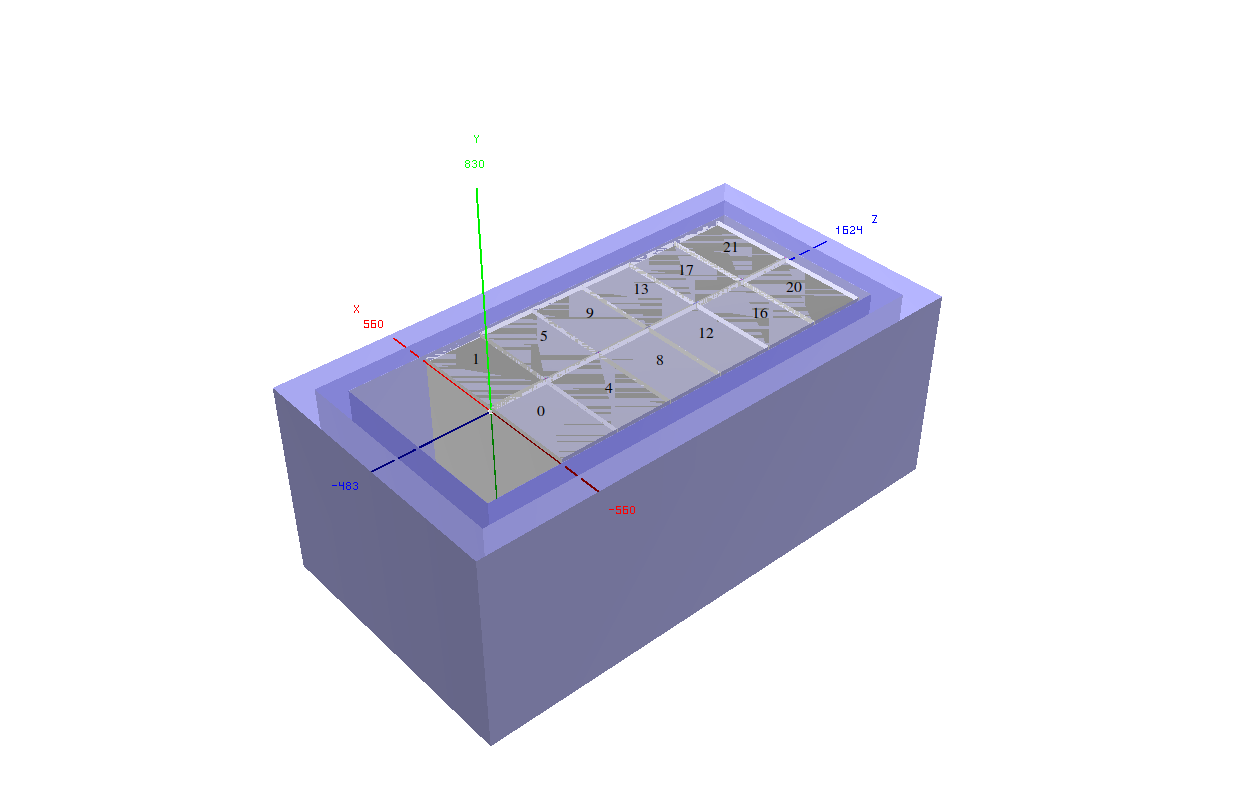
\includegraphics[width=\linewidth]{graphics/duneworkspace126_lowerhalf_numbered.png}
    \caption{Perspective view of the 1x2x6 configuration.}
    \label{fig:my_label}
\end{figure}
From the geometry documentation, the layout is written:
\begin{code}{text}
Plan view, from the top, of the lower 12 TPCs, 
shown inside the TPC volumes.  
The beam enters from the left.

   ----------------- -----------------  CPA

     1     5     9    13    17    21
   ===== ===== ===== ===== ===== =====  APA
     0     4     8    12    16    20

   ------------------ ----------------  CPA

Plan view, from the top, of the upper 12 TPCs, 
shown inside the TPC volumes.  
The beam enters from the left.

   ----------------- -----------------  CPA

     3     7    11    15    19    23
   ===== ===== ===== ===== ===== =====  APA
     2     6    10    14    18    22

   ------------------ ----------------  CPA
\end{code}
which shows that there are 24 TPC volumes in a 2x2x6 formation, with an APA (Anode plane assembly) separating the TPCs down the middle (z axis).  More information about this geometry can be found in the \hyperref[1x2x6appendix]{Appendix}.  There are some global values which will be useful to list here, such as the dimensions of the active TPC volume for the entire detector:
\begin{table}[H]
    \centering
    \begin{tabular}{|c|c|c|c|}
    \hline
        \multicolumn{4}{|c|}{\textbf{Horizontal Drift 1x2x6 v4 refactored}}\\
        \hline
        Volume & \makecell{X ranges (cm)\\ \[min,max\]} & \makecell{Y ranges\\cm} & \makecell{Z ranges\\cm}\\
        \hline
        \hline
        World & \makecell{[-3609.66,\\  3609.66]} & \makecell{[-3908.85,\\  3908.85]} & \makecell{[-4153.24,\\  4153.24]}\\
        \hline
        Cryostat &\makecell{[-379.662,\\  379.662]} & \makecell{[-658.099,\\  699.599]} & \makecell{[-302.946,\\  1443.53]} \\
        \hline
        TPC (full) &\makecell{[-363.376,\\  363.376]} & \makecell{[-607.829,\\  607.829]} & \makecell{[-0.87625,\\  1393.46]} \\
        \hline
        TPC ({\color{red}active}) & \makecell{[-363.376,\\  363.376]} & \makecell{[-600.019,\\  600.019]} & \makecell{[-0.87625,\\  1393.46]} \\
        \hline
    \end{tabular}
    \caption{Geant4 volume information for the horizontal drift 1x2x6 version 4 refactored geometry.}
    \label{tab:my_label}
\end{table}

\subsection{The Simulation Chain}
The simulation chain involves a distinct set of steps which can be broken down into the following pieces:
\begin{enumerate}
    \item \textbf{generator} - this stage generates the initial four vectors for particles in an event.
    \item \textbf{g4} - the g4, or Geant4, step simulates the particles traversing the detector volume which includes interactions that produce daughter particles and deposits of energy.
    \item \textbf{detsim} - detsim, or detector simulation, involves simulating the detector response, e.g. the drift of electrons to wires and their response to the charges (this step is supposed to generate output which is in an identical form to what is read from the physical detector).
    \item \textbf{reco} - the reco step consists of a set of tools for reconstructing events from the detsim output to various ``truth'' values.
\end{enumerate}
The next few sections will detail each of the steps described above.  If one is only interested in running the code, skip to \hyperref[runningthecode]{section ...}  


\subsection{The Generator Step}
The generator step involves only a couple of things to consider and in general is the simplest of the entire simulation chain.
\paragraph{Generating input files ---}First, we must generate some input files to use in our simulation.  These will consist of a specification of particles with a particular initial momentum, total energy, mass and position.  In our case, these particles will be neutrons (PDG code 2112) which if coming from a PNS (i.e. the DDG), is assumed to be mono-energetic -- they all have the same total energy and hence the same total momentum.  We can generate these events with a helper script written in python, ``PNS\_generator.py'', which has the following function:
\begin{code}{python}
generate_ddg_neutrons(
    50,         # number of events to generate 
    1450,       # number of neutrons to generate per event 
    0.057,      # magnitude of the initial momentum in GeV 
    .939,       # total initial energy of the neutrons in GeV 
    0,          # x position of the source in cm
    0,          # y position of the source in cm
    700,        # z position of the source in cm
    "test.dat", # file to output the results to     
    False,      # check1: momentum direction check
    True        # check2: momentum magnitude check
)
\end{code}
The first check (which is set to False above) will generate a plot of the momentum directions, which allows one to see if they have been correctly been generated uniformly on a sphere of radius $|\vec{p}|$.  An example is shown below:
\begin{figure}[H]
    \centering
    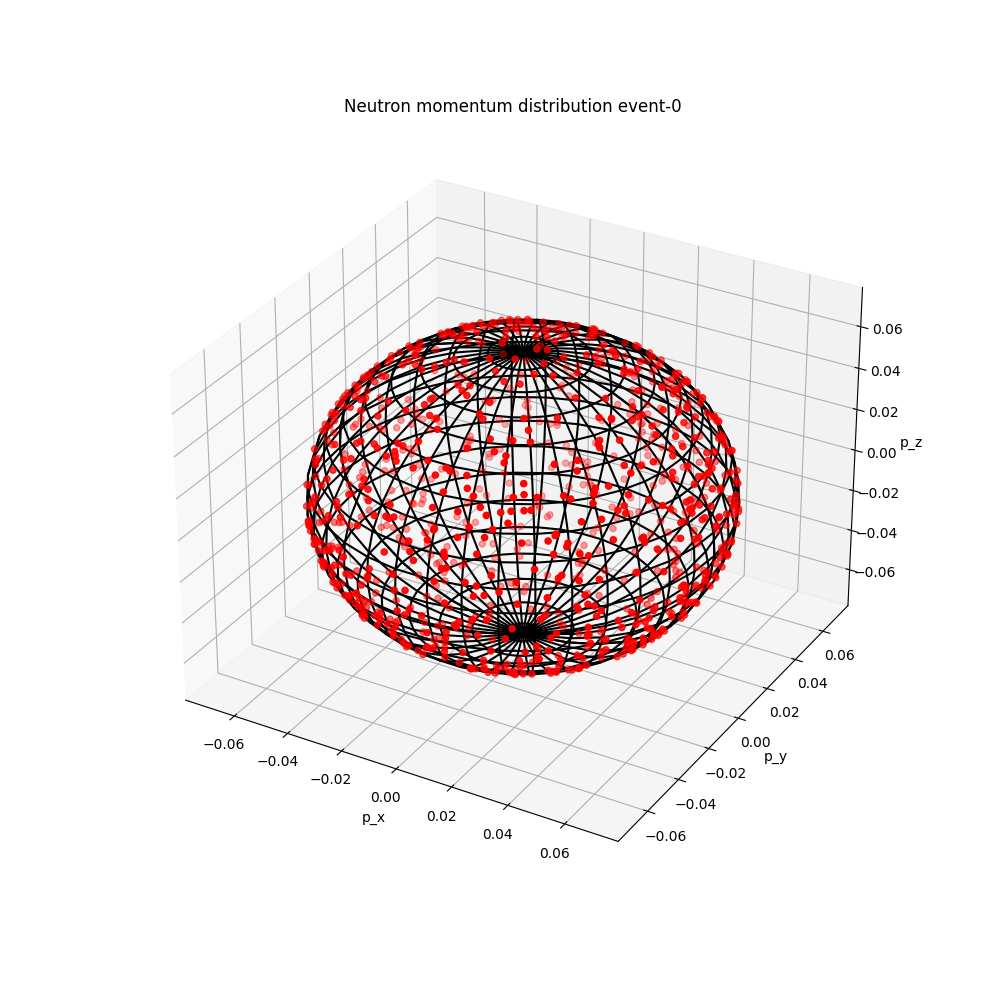
\includegraphics[width=\linewidth]{graphics/Argon_sphere_1_1000_0.0024995794800000137.dat-event-0.png}
    \caption{Distribution of the momenta, on a sphere of constant magnitude, of particles generated with the \textit{PNS\_generator.py} script.}
    \label{fig:momenta_distribution}
\end{figure}
The second check sums the squared differences between the simulated momentum magnitudes and the desired magnitude and prints out the results for each event.  This function will generate a .dat file in HEPevt format, which is described in the next section.

\index{HEPevt}\marginlabel{HEPevt format:}The .dat files used to specify the DDG neutrons in the generator step are in HEPevt\footnote{HEPevt format, or \textit{high energy physics event format}, is a standard that was agreed upon during the 1989 LEP physics study \cite{LEP89}.  For more info see \href{https://home.fnal.gov/~mrenna/lutp0613man2/node49.html}{this page}.} format and contain the following information (with a DDG neutron as an example):
\begin{table}[H]
    \centering
    \begin{tabular}{|c|c|}
        \hline
         NEVHEP (Event Number) & NHEP (Number of particles in the event) \\
         \hline
         \hline
         0 & 1450\\
         \hline
    \end{tabular}
    \caption{Example of the beginning of an event record in HEPevt format.  Each new event record consists of two values, the event number (NEVHEP) which starts from 0, and the number of particles simulated for that event (NHEP).  In the example above, we are generating event zero which will produce 1450 particles.}
    \label{tab:my_label}
\end{table}
The next NHEP lines after each event header contains the individual particle information for each particle.  The first six values in each record are the following:
\begin{table}[H]
\centering
\begin{tabular}{|l|c|r|}
    \hline
     Abbrv. & Descrip. & Example\\
     \hline
     \hline
     ISHEP &  particle status & 1 (final state)\\
     \hline
     IDHEP (PDG) & PDG Code & 2112 (neutron)\\
     \hline
     JMOHEP1 & 1st mother & 0\\
     \hline
     JMOHEP2 & 2nd mother & 0\\
     \hline
     JDAHEP1 & 1st daughter & 0\\
     \hline
     JDAHEP2 & 2nd daughter & 0\\
     \hline
     PHEP1 & $p_x$ (GeV) & -0.00626188\\
     \hline
     PHEP2 & $p_y$ (GeV) & 0.012882\\
     \hline
     PHEP3 & $p_z$ (GeV) & -0.00626188\\
     \hline
     PHEP4 & $E_{\mathrm{tot}}$ (GeV) & 0.942065\\
     \hline
     PHEP5 & $m$ (GeV) & 0.939656 (neutron)\\
     \hline
     VHEP1 & $x_i$ (mm)& 355\\
     \hline
     VHEP2 & $y_i$ (mm)& 630\\
     \hline
     VHEP3 & $z_i$ (mm)& 60\\
     \hline
     VHEP4 & $t_{\mathrm{production}}$ (mm/c) & 0\\
     \hline
\end{tabular}
\caption{Example of a particle event record in HEPevt format, where ISHEP is an integer code identifying the particle status and IDHEP is the particle’s PDG code.  The JMOHEP1, JMOHEP2, JDAHEP1, and JDAHEP2 entries record the indices (between 1 and NHEP, inclusive) of particles in the event record that correspond to the first mother, second mother, first daughter, and last daughter of the current particle, respectively. These indices are set to zero in cases where they do not apply (e.g., a particle with no daughters will have JDAHEP1 = JDAHEP2 = 0). Entries PHEP1 through PHEP3 record the x-, y-, and z-components of the particle 3-momentum, while PHEP4 gives the total energy and PHEP5 gives the particle mass (all in GeV). Entries VHEP1 through VHEP3 store the x, y, and z positions of the particle production vertex (mm), and VHEP4 gives the production time (mm/c).  Info about HEPevt format is taken from \url{http://www.marleygen.org/interpret_output.html}.}
\end{table}

\paragraph{Generator Producers ---}
The generator step has the following producers:
\begin{code}{perl}
physics:
{
    producers:  
    {
        generator:       @local::standard_textfilegen
        ar39:            @local::dune10kt_1x2x6_39ar
        rns:             { module_type: "RandomNumberSaver" }
    }
    simulate: [generator, ar39, rns]
    stream1:  [ out1 ]
    trigger_paths: [simulate] 
    end_paths:     [stream1]  
}
\end{code}
The standard text-file generator is what takes in our neutron information from the .dat file we produced in the previous step.  The Ar39 generator is defined in ``dune\_radiological\_model.fcl'', which has the following specifications:
\begin{code}{perl}
dune10kt_1x2x6_39ar:
{
 module_type:  "RadioGen"
 Nuclide:   [ "39Ar" ]    # list of nuclides to simulate, supported so far: 39Ar, 60Co, 85Kr, 40K, 232Th, 238U, 222Rn
 Material:  ["LAr"]
 BqPercc:   [ 0.00141 ]   # activity -- Becquerels per cc. 0.00141 assumes 1.01 Bq/kg (typical for 39Ar) and a density of 1.396 g/cc for LAr
 X0:        [ -475. ]     # in cm in world coordinates, bottom corner of box
 X1:        [  475. ]     # in cm in world coordinates, top corner of box
 Y0:        [ -750. ]     # in cm in world coordinates, bottom corner of box
 Y1:        [  800. ]     # in cm in world coordinates, top corner of box
 Z0:        [  -55. ]     # in cm in world coordinates, bottom corner of box
 Z1:        [  1500. ]     # in cm in world coordinates, top corner of box
 T0:        [ -2246000 ]
 T1:        [  2246000. ] # ending time in ns
}
\end{code}

\paragraph{Generator Services ---}

\subsection{The Geant4 Step}

\index{MCParticle}\marginlabel{MCParticle:}LArSoft saves most of the information coming from Geant4 particles into a class called \href{https://internal.dunescience.org/doxygen/classsimb_1_1MCParticle.html}{simb::MCParticle} which is in the \href{https://internal.dunescience.org/doxygen/namespacesimb.html}{simb} (simulation base) namespace.  This class keeps track of many things, such as the four-position and four-momentum for each time step, as well as mother and daughter particle information\footnote{One thing to keep in mind is that certain processes in Geant4 cause incoming particles to be destroyed, and new identical particles to be put in their place.  For example, in an inelastic scattering of a neutron with a nucleus, if the neutron continues in an altered trajectory, Geant4 will assign it to a new particle, rather than updating the state of the old particle.  This can be quite annoying, however in LArSoft you can easily identify these transfers by matching the ID of the \textit{mother} of a particle, with the \textit{TrackID} of the mother itself. In other words, if particle one (p1) is the incident particle and particle two (p2) is the same particle but outgoing, then we could have, \textit{p1.TrackId() = p2.Mother()}.}.  It also keeps track of process which created the particle, as well as the ending process.  You can also extract information about where the particle is in the detector by using it's position at a given time step, and asking for the detector properties at that position, e.g.:
\begin{code}[1][Basic functionality for extracting geometry information from LArSoft.  Once you've constructed a service handle using \href{https://internal.dunescience.org/doxygen/classart_1_1ServiceHandle.html}{art::ServiceHandle} for a \href{https://internal.dunescience.org/doxygen/classgeo_1_1Geometry.html}{geo::Geometry} object, one can then grab material information using the \href{https://root.cern/doc/master/classTGeoMaterial.html}{TGeoMaterial} class, or by using the many methods from \href{https://internal.dunescience.org/doxygen/classgeo_1_1GeometryCore.html}{geo::GeometryCore}.]{c++}
// possible includes you will need
#include "art/Framework/Services/Registry/ServiceHandle.h"
#include "larcore/Geometry/Geometry.h"
#include "larcorealg/Geometry/GeometryCore.h"
#include "TGeoMaterial.h"
#include "TGeoElement.h"
// geometry services
art::ServiceHandle<geo::Geometry> geometryService;
geo::GeometryCore const* geometryCore;
geometryCore = lar::providerFrom<geo::Geometry>();
// material objects (TGeoMaterial is from ROOT)
const TGeoMaterial *material;
geo::Point_t materialPOI;
.
.
.
// later in your "analyze" method...
// check the current material
double mc_x = ...
materialPOI.SetCoordinates(mc_x,mc_y,mc_z);
material = geometryService->Material(materialPOI);
// get the eff. atomic number at the POI
double eCode = material->GetZ();
// get the name of the deepest volume at the POI
std::string vol = geometryService->VolumeName(materialPOI);
\end{code}


\subsection{The Detector Simulation Step}

\subsection{The Standard Reconstructions Step}

\subsection{Running the Code}\label{runningthecode}
In order to make sure that everything is working correctly, we will run some simple examples which only contain a few neutrons for each event.
\subsubsection{Example 1: A single neutron}
We will play with generating a single neutron at the center of the 1x2x6 geometry and see whether we can find a neutron capture on the LAr. To begin, we will generate 5000 events, each with a single neutron.  We can do this by running the following script in the ``examples/single\_neutron/'' folder:
\begin{code}{shell}
python3 generate_center_of_1x2x6.py
\end{code}
which should quickly pump out a file named
\begin{code}{text}
example\_single\_neutron\_1x2x6.dat
\end{code}
This can then be fed into the generator step by running
\begin{code}{shell}
lar -c example_single_neutron_1x2x6_generator.fcl
\end{code}
which itself will produce an output called
\begin{code}{text}
example\_single\_neutron\_1x2x6\_generator\_output.root
\end{code}



\newpage 
\section{Neutron Calibration in the Single Phase Vertical Drift Far Detector (FDVD)}


\index{DUNE geometries!Vertical Drift}\subsection{Geometries}


\index{DUNE geometries!Vertical Drift!1x6x6}\marginlabel{1x6x6 geometry:}
There are some global values which will be useful to list here, such as the dimensions of the active TPC volume for the entire detector:
\begin{table}[H]
    \centering
    \begin{tabular}{|c|c|c|c|}
        \hline
        \multicolumn{4}{|c|}{\textbf{Vertical Drift 1x6x6 two-view v1 refactored}}\\
        \hline
        Volume & \makecell{X ranges (cm)\\ \[min,max\]} & \makecell{Y ranges\\cm} & \makecell{Z ranges\\cm}\\
        \hline
        \hline
        World & \makecell{[-4655.14,\\  4655.14]} & \makecell{[-4886.34,\\  4886.34]} & \makecell{[-4827.97,\\  4827.97]}\\
        \hline
        Cryostat &\makecell{[-425.12,\\  425.16]} & \makecell{[-606.34,\\  606.34]} & \makecell{[-100.17,\\  995.774]} \\
        \hline
        TPC (full) &\makecell{[-325.00,\\  325.04]} & \makecell{[-506.22,\\  506.22]} & \makecell{[-0.05,\\  895.654]} \\
        \hline
        TPC ({\color{red}active}) & \makecell{[-325.00,\\  325.00]} & \makecell{[-506.17,\\  506.17]} & \makecell{[0.00,\\  895.604]} \\
        \hline
    \end{tabular}
    \caption{Geant4 Volumes defined for the Vertical Detector 2-view v1 refactored 1x6x6 geometry.}
    \label{tab:my_label}
\end{table}

\subsection{The Simulation Chain}

The next few sections will detail each of the steps described above.  If one is only interested in running the code, skip to \hyperref[runningthecode]{section ...}  



\subsection{The Generator Step}



\paragraph{Generator Producers ---}


\paragraph{Generator Services ---}

\subsection{The Geant4 Step}



\subsection{The Detector Simulation Step}

\subsection{The Standard Reconstructions Step}

\subsection{Running the Code}\label{runningthecode}




\newpage


\printbibliography

\newpage
\appendix

\section{FNAL Computing Environment}
\subsection{Unix Product Service}
To see which UPS commands are available, simply enter ``ups'' in the console, and it will generate the following list:
\begin{code}{text}
UPS commands:

for specific command options use "ups COMMAND -?"

          configure   : Environmentally configure a product instance.
          copy        : Allow one instance of a product to be declared 
                        "like" another.
          declare     : Add a product instance or a chain to a UPS Database.
          depend      : List (for a specified UPS product instance) 
                        UPS product requirements or all UPS product instances 
                        which this product depends upon
          exist       : Determine if a setup command with the same options 
                        would likely succeed.
          flavor      : Print flavor of a machine, optionally by 
                        level, or table generated for searching
          get         : Return a list of all files that are needed 
                        by a product instance and do not live under 
                        the product root directory.
          help        : Output help information for all UPS commands
          list        : List UPS Database information about product instances.
          layout      : Show type of layout for databases.
          modify      : Allow editor modification of the UPS Database files.  
                        The altered files are verified before being rewritten.
          parent      : List products which depend on specified product instances.
          setup       : Prepare the environment in order to be able 
                        to use a product instance.
          start       : Perform any necessary actions for a product 
                        instance at system boot.
          stop        : Perform any necessary actions for a product 
                        instance at system shutdown.
          tailor      : Perform any product instance tailoring that needs 
                        to be done once (specify hardware device location)
                        or needs user input.
          touch       : Will change a ups file modify time (MODIFIED) to current time
                        (it will probably also change the modifier (MODIFIER)).
          unconfigure : Undo any actions performed by the configure command.
          undeclare   : Remove a product instance from a UPS Database. 
                        if chain(s) are specified ONLY the chain(s) will 
                        be removed if a version is specified ALL chain and 
                        version will be removed
          unsetup     : Return the environment to a pre-setup state.
          verify      : Check the specified instances for correct formatting 
                        and information.
\end{code}

\section{Scripts}
\subsection{Neutron Analyzer}\label{fnalsetupscript}
\begin{code}{bash}
# environment variables
# if you change the larsoft version, or the quals, you
# must check for the appropriate artg4tk version.  This can
# be done by issuing: ups depend larsoft <VERSION> -q <QUALS> | grep "artg4tk"
INSTALL_DIRECTORY = /dune/app/users/$USER/NeutronCalibrationLArSoft
LARSOFT_VERSION   = v09_31_00
DUNETPC_VERSION   = v09_31_00
ARTG4TK_VERSION   = v10_03_00
QUALS             = e20:prof
echo "Installing a new custom LArSoft build with "
echo "INSTALL_DIRECTORY = {$INSTALL_DIRECTORY}"
echo "LARSOFT_VERSION   = {$LARSOFT_VERSION}"
echo "DUNETPC_VERSION   = {$DUNETPC_VERSION}"
echo "ARTG4TK_VERSION   = {$ARTG4TK_VERSION}"
echo "QUALS             = {$QUALS}"
echo "Setting up UPS..."
source /cvmfs/dune.opensciencegrid.org/products/dune/setup_dune.sh
echo "Setting up LArSoft version={$LARSOFT_VERSION} quals={$QUALS}..."
setup larsoft $LARSOFT_VERSION -q $QUALS
echo "Setting up ninja..."
setup ninja
echo "Creating installation directory..."
mkdir $INSTALL_DIRECTORY
cd $INSTALL_DIRECTORY
echo "Setting up new MRB development environment..."
mrb newDev
source localProducts*/setup
cd $MRB_SOURCE
echo "Collecting dunetpc and artg4tk..."
mrb g -t $DUNETPC_VERSION dunetpc
mrb g -t $ARTG4TK_VERSION artg4tk
cd dunetpc/dune/
echo "Collecting NeutronAnalyzer..."
git clone https://github.com/infophysics/NeutronAnalyzer
echo "add_subdirectory(NeutronAnalyzer)" | tee -a CMakeLists.txt
cd $MRB_BUILDDIR
echo "Installing..."
mrbsetenv
mrb install -j 32 --generator ninja
\end{code}

\section{Geometries}

\subsection{1x2x6 Geometry}\label{1x2x6appendix}
Using the various classes in the \href{https://internal.dunescience.org/doxygen/classgeo_1_1GeometryCore.html}{geo::GeometryCore} class, we can extract the following information from the \hre{}{fourth version of the refactored geometry}:

% \begin{landscape}
% \begin{flushleft}

% \begin{minipage}[t]{.8\textheight}
\Rotatebox{90}
{
    \centering
    \begin{tabular}{|c|c|c|c|c|c|c|c|}
        \hline
        \# & (X,Y,Z) center (cm) & \makecell{X min\\full/{\color{red}active}} & \makecell{X max\\full/{\color{red}active}} & \makecell{Y min\\full/{\color{red}active}} & \makecell{Y max\\full/{\color{red}active}} & \makecell{Z min\\full/{\color{red}active}} & \makecell{Z max\\full/{\color{red}active}} \\
        \hline
        \hline
         0 &  (-182.955,-303.914,115.319) & -363.376/{\color{red}*} & -2.53305/{\color{red}-3.96105} & -607.829/{\color{red}-600.019} & 0/{\color{red}*} & -0.87625/{\color{red}*} & 231.514/{\color{red}*}\\
         \hline
         1 &(182.955,-303.914,115.319)& & & & & &  \\
         \hline
         2 &(-182.955,303.914,115.319)& & & & & &  \\
         \hline
         3 &(182.955,303.914,115.319)& & & & & &  \\
         \hline
         4 &(-182.955,-303.914,347.709)& & & & & &  \\
         \hline
         5 &(182.955,-303.914,347.709)& & & & & &  \\
         \hline
         6 &(-182.955,303.914,347.709)& & & & & &  \\
         \hline
         7 &(182.955,303.914,347.709)& & & & & &  \\
         \hline
         8 &(-182.955,-303.914,580.099)& & & & & &  \\
         \hline
         9 &(182.955,-303.914,580.099)& & & & & &  \\
         \hline
         10 &(-182.955,303.914,580.099)& & & & & &  \\
         \hline
         11 &(182.955,303.914,580.099)& & & & & &  \\
         \hline
         12 &(-182.955,-303.914,812.489)& & & & & &  \\
         \hline
         13 &(182.955,-303.914,812.489)& & & & & &  \\
         \hline
         14 &(-182.955,303.914,812.489)& & & & & &  \\
         \hline
         15 &(182.955,303.914,812.489)& & & & & &  \\
         \hline
         16 &(-182.955,-303.914,1044.88)& & & & & &  \\
         \hline
         17 &(182.955,-303.914,1044.88)& & & & & &  \\
         \hline
         18 &(-182.955,303.914,1044.88)& & & & & &  \\
         \hline
         19 &(182.955,303.914,1044.88)& & & & & &  \\
         \hline
         20 &(-182.955,-303.914,1277.27)& & & & & &  \\
         \hline
         21 &(182.955,-303.914,1277.27)& & & & & &  \\
         \hline
         22 &(-182.955,303.914,1277.27)& & & & & &  \\
         \hline
         23 &(182.955,303.914,1277.27)& & & & & &  \\
        \hline
    \end{tabular}

}
% \end{minipage}
% \end{flushleft}
% \end{landscape}

\printindex

\end{document}

